\documentclass[12pt]{article}
\usepackage[utf8]{inputenc}
\usepackage{graphicx} % Required for inserting images
\usepackage{amsmath,amsfonts,amssymb}
\usepackage{algorithm}
\usepackage{algpseudocode}
\usepackage{cite}
\usepackage{url}
\usepackage{booktabs}
\usepackage{graphicx}
\usepackage{caption}
\usepackage{tikz}
\usetikzlibrary{shapes, arrows.meta, positioning, decorations.pathreplacing}
\usepackage[colorlinks]{hyperref}
\usepackage{xcolor}
\usepackage[margin=1in]{geometry}

\setlength{\parskip}{1em}
\setlength{\parindent}{0em}
\setcounter{page}{1}

\title{Modeling Regional Infectious Disease Spread with Physics-Informed Neural Networks: A Study on COVID-19 Dynamics}
\author{Michael Ajao-olarinoye \\
    center for computational science and mathematical modelling \\
    coventry university \\
    \url{olarinoyem@coventry.ac.uk}}
\date{}

\begin{document}

\maketitle

\begin{abstract}
    The COVID-19 pandemic has presented numerous challenges to healthcare systems globally, particularly in managing the demand for critical resources such as mechanical ventilators. Accurate forecasting of ventilator demand is paramount to ensure effective resource allocation and preparedness. This study employs a novel approach by integrating Universal Differential Equations (UDE) within a SEIR-based epidemiological model to forecast the demand for mechanical ventilators in England using real-world COVID-19 data. Our model uniquely blends data-driven machine learning components with traditional epidemiological modeling, allowing for a nuanced understanding of disease transmission dynamics and healthcare resource utilization. Utilizing data on daily case counts, hospital admissions, and mechanical ventilator usage over time, we trained neural network components to estimate key parameters dynamically. Our results indicate that the UDE-based model provides robust short-term forecasts of ventilator demand, aiding in timely resource allocation and policy interventions. This approach showcases the potential of hybrid modeling techniques in enhancing healthcare system preparedness and response during public health crises.
\end{abstract}

\section{Introduction}

The virus SARS-COV-2 causes COVID-19, a severe respiratory disease with a high mortality rate that has triggered a global pandemic \cite{forman202012}. The disease have affected more than 210 countries and territories, infecting hundreds of millions of people and killing millions. COVID-19 poses a complex and unprecedented challenge for public health and society, requiring scientific efforts to understand, model, diagnose and control the virus and disease. The COVID-19 pandemic has strained healthcare systems worldwide, requiring effective resource allocation and intervention strategies to mitigate the virus's impact \cite{emanuel2020fair}. Resource allocation is the process of distributing and allocating resources, which can include financial and non-financial assets, to achieve specific objectives or goals \cite{jiang2019emergency}. Resource allocation interventions for the COVID-19 pandemic can be divided into pharmaceutical and non-pharmaceutical interventions \cite{ehmann2021operational}. For instance, in healthcare systems, resource allocation may include both pharmaceutical resources, such as medications and vaccines, and non-pharmaceutical resources, such as ICU beds, medical equipment and personnel, to ensure effective and efficient delivery of healthcare services \cite{zaric2001resource, brandeau2004allocating}. Current studies often focus on the allocation of a single type of resource, such as pharmaceutical or non-pharmaceutical resources. However, in reality, resource allocation often involves multiple types of resources that are interrelated and have different allocation principles. Epidemiological modelling and resource demand forecasting are essential for informing resource allocation decisions. These models use data on various factors, such as disease prevalence, population demographics, and healthcare capacity, to predict the demand for different types of resources.

These will help in developing strategies for disease prevention and control, as well as sustainable public health policies and economic activity guidelines. Mathematical models have always been useful in understanding the transmission mechanisms of a disease outbreak and providing valuable insights for controlling it. 

There are different ways to model infectious diseases like covid-19. One way is to count the number of people who are infected, recovered, dead, or susceptible in an epidemic. This is called the compartmental model, and it is the most popular mathematical model that researchers use to study the disease. The compartmental model can be either deterministic or stochastic. Deterministic models can simulate a general scenario of how the disease spreads. Stochastic models can simulate how the disease spreads in small or sub-grouped populations, or predict the possible outcomes. Other mathematical models have also been used to describe infectious disease, such as in

\section{literature review}




\section{Methodology}
This section describes the methodology used in this study. It includes the data collection, data preprocessing, model development, and model evaluation.
\subsection{mathematical modeling of infectious disease}
In the context of the COVID-19 pandemic, accurate epidemiological modelling and resource demand forecasting play a crucial role in informing healthcare professionals and governments on how to effectively manage the overburdened healthcare systems. The use of predictive models has been crucial in the context of the COVID-19 pandemic, aiding healthcare professionals and governments in effectively managing the overburdened healthcare systems. The most common model is the Susceptible-Infectious-Removed (SIR) epidemic model. It was proposed by Kermack-Mckendrick in 1927 \cite{kermack1927contribution}. 

\subsection{SIR and SEIRD models}
The SIR and SEIRD models are pivotal in understanding the dynamics of infectious diseases, such as COVID-19, providing insights into how diseases spread and recede within populations. These models help in predicting the number of individuals affected by a disease over time and are crucial for public health planning and intervention strategies.

The SIR model compartmentalizes the population into three categories: Susceptible (S), Infectious (I), and Recovered (R) individuals. The transitions between these categories are governed by a set of ordinary differential equations (ODEs) as follows:

\begin{equation}
\frac{dS}{dt} &= -\beta \frac{SI}{N}, \\
\frac{dI}{dt} &= \beta \frac{SI}{N} - \gamma I, \\
\frac{dR}{dt} &= \gamma I,
\end{equation}

where $S$ represents the number of susceptible individuals who are not yet infected but can be, $I$ denotes the number of infectious individuals who can transmit the disease to susceptible individuals and recover, and $R$ represents the number of recovered individuals who are immune to the disease. The parameters $\beta$ and $\gamma$ represent the transmission rate and recovery rate, respectively. The total population size is denoted by $N = S + I + R$. The SIR model is a simple and effective tool for understanding the dynamics of infectious diseases and has been widely used to model the spread of various diseases, including COVID-19.

\begin{tabular}{ll}
    \toprule
    \textbf{Parameter} & \textbf{Definition} \
    \midrule
    $\beta$ & Transmission rate \
    $\gamma$ & Recovery rate \
    \bottomrule
\end{tabular}
    
The SIR model is fundamental in epidemiology for its simplicity and effectiveness in capturing the basic dynamics of disease spread. However, it assumes lifelong immunity post-recovery, which may not apply to all diseases, including COVID-19.
\begin{figure}[h!]
    \centering
    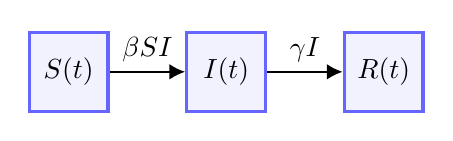
\begin{tikzpicture}[node distance=2cm, auto, thick]
        % Define block styles
        \tikzstyle{block} = [rectangle, draw=blue!60, fill=blue!5, very thick, minimum size=1cm, text centered]
        \tikzstyle{line} = [draw, -{Latex[length=2mm, width=2mm]}]

        % Define nodes
        \node [block] (S) {\( S(t) \)};
        \node [block, right of=S] (I) {\( I(t) \)};
        \node [block, right of=I] (R) { \( R(t) \)};

        % Connect nodes with paths
        \path [line] (S) -- node { \( \beta S I \) } (I);
        \path [line] (I) -- node { \( \gamma I \) } (R);

    \end{tikzpicture}
    \caption{Compartmental flow of the SIR model for infection transmission dynamics.}
\end{figure}

To account for the characteristics of COVID-19, including the existence of a latent period and the possibility of death, the SEIRD model extends the SIR framework by including two additional compartments: Exposed (E) and Dead (D) individuals. The SEIRD model is described by the following differential equations:

\begin{equation}
\frac{dS}{dt} &= -\beta \frac{SI}{N}, \\
\frac{dE}{dt} &= \beta \frac{SI}{N} - \sigma E, \\
\frac{dI}{dt} &= \sigma E - \rho I - \alpha I, \\
\frac{dR}{dt} &= \rho I, \\
\frac{dD}{dt} &= \alpha I,
\end{equation}

where $E$ represents the number of exposed individuals who are infected but not yet infectious, and $D$ represents the number of deceased individuals. The parameters $\sigma$, $\rho$, and $\alpha$ represent the rate of exposed individuals becoming infectious, the recovery rate, and the mortality rate, respectively. The total population size is denoted by $N = S + E + I + R + D$. The SEIRD model provides a more comprehensive representation of disease dynamics and is particularly useful for capturing the spread of COVID-19, which exhibits a latent period and the possibility of death. This model more accurately reflects the disease dynamics of COVID-19 by considering the exposed phase, during which individuals are infected but not yet infectious, and the mortality due to the disease. The addition of these compartments allows for a more nuanced understanding of the pandemic's progression and the impact of interventions such as social distancing, vaccination, and treatment strategies.


\begin{figure}[h!]
    \centering
    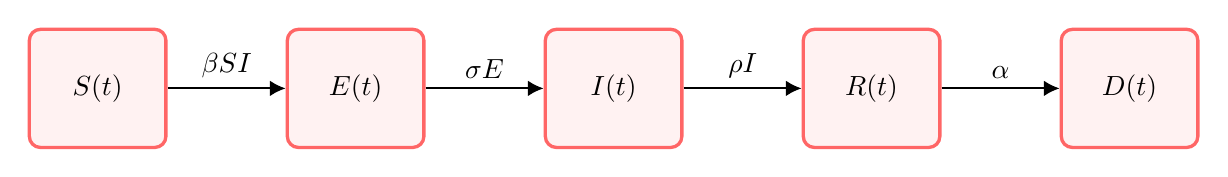
\begin{tikzpicture}[node distance=1.5cm, auto, thick]
        % Define block styles
        \tikzstyle{roundnode} = [circle, draw=green!60, fill=green!5, very thick, minimum size=1cm, text centered]
        \tikzstyle{squarednode} = [rectangle, draw=red!60, fill=red!5, very thick, text width=1.5cm, text centered, rounded corners, minimum height=1.5cm]
        \tikzstyle{line} = [draw, -{Latex[length=2mm, width=2mm]}]
    
        % Define nodes
        \node [squarednode] (S) {\( S(t) \)};
        \node [squarednode, right=of S] (E) {\( E(t) \)};
        \node [squarednode, right=of E] (I) {\( I(t) \)};
        \node [squarednode, right=of I] (R) { \( R(t) \)};
        \node [squarednode, right=of R] (D) { \( D(t) \)};
        
        % Connect nodes with paths
        \path [line] (S) -- node { \( \beta S I \) } (E);
        \path [line] (E) -- node { \(  \sigma E \) } (I);
        \path [line] (I) -- node { \( \rho I\) } (R);
        \path [line] (R) -- node { \( \alpha \) } (D);

    \end{tikzpicture}
    \caption{Compartmental flow of the SEIRD model for COVID-19 transmission dynamics.}
\end{figure}



\section{Results and Discussion}





\section{Conclusion}




\begin{algorithm}
\caption{Physics-Informed Neural Network (PINN) Training for Epidemic Modeling}
\begin{algorithmic}[1]
\Require Training data tensors $S_{data}$, $I_{data}$, $R_{data}$, Time tensor $t_{data}$, Population $N$, Neural Network $NN$ with weights $w$ and biases $b$
\Ensure Preprocessed tensors on the same device
\State Initialize $NN$ with Xavier initialization for weights $w$ and biases $b$
\State Define early stopping criteria with patience and delta
\State Set learning rate $lr$ and regularization parameters $\lambda$, $p$

\For{each epoch up to $num\_epochs$}
    \State Compute predictions: $S_{pred}$, $I_{pred}$, $R_{pred} \gets NN(t_{data})$
    \State Compute time derivatives of $S_{pred}$, $I_{pred}$, $R_{pred}$ via autograd
    \State Calculate residuals using SIR model equations:
    \begin{align*}
    \frac{dS}{dt} & = -\beta \frac{S_{pred} I_{pred}}{N} \\
    \frac{dI}{dt} & = \beta \frac{S_{pred} I_{pred}}{N} - \gamma I_{pred} \\
    \frac{dR}{dt} & = \gamma I_{pred}
    \end{align*}
    \State Compute loss function components:
    \State $MSE_{SIR} \gets \frac{1}{q} \sum_{i=1}^{q} \left[ \left(S_{i} - S_{pred_i}\right)^2 + \left(I_{i} - I_{pred_i}\right)^2 + \left(R_{i} - R_{pred_i}\right)^2 \right]$
    \State $MSE_{residuals} \gets \frac{1}{q} \sum_{i=1}^{q} \left[ \left(\frac{dS_i}{dt} - \frac{dS_{pred_i}}{dt}\right)^2 + \left(\frac{dI_i}{dt} - \frac{dI_{pred_i}}{dt}\right)^2 + \left(\frac{dR_i}{dt} - \frac{dR_{pred_i}}{dt}\right)^2 \right]$
    \State $Loss \gets MSE_{SIR} + MSE_{residuals} + \lambda \cdot \text{Regularization}(NN)$
    \State Update $NN$ parameters via backpropagation and optimization step
    \State Adjust learning rate with learning rate scheduler if needed
    \State Check for early stopping, break if condition is met
\EndFor

\State \textbf{Output:} Trained PINN model $NN$
\end{algorithmic}
\end{algorithm}


\begin{algorithm}
\caption{Training of Physics-Informed Neural Network (PINN) for Epidemic Modeling}
\begin{algorithmic}[1]
\Require Training data tensors $\bm{S}_{data}$, $\bm{I}_{data}$, $\bm{R}_{data}$, time tensor $\bm{t}_{data}$, population size $N$, initial learning rate $lr$, regularization parameters $\lambda_{reg}$, $p_{reg}$, and number of epochs $num\_epochs$.
\Ensure All tensors are on the computational device, e.g., GPU.
\State Initialize PINN $NN$ with weights $\bm{w}$ and biases $\bm{b}$ using Xavier initialization.
\State Define EarlyStopping class with patience, delta, and verbose output.
\State Set up the Adam optimizer with learning rate $lr$ and weight decay.
\State Set up learning rate scheduler with reduction factor and patience.

\For{$epoch = 1$ to $num\_epochs$}
    \State Compute predictions $\bm{S}_{pred}$, $\bm{I}_{pred}$, $\bm{R}_{pred}$ from $NN(\bm{t}_{data})$.
    \State Compute gradients $\frac{d\bm{S}_{pred}}{dt}$, $\frac{d\bm{I}_{pred}}{dt}$, $\frac{d\bm{R}_{pred}}{dt}$ with respect to $\bm{t}_{data}$ using automatic differentiation.
    
    \State Define the SIR model's theoretical dynamics:
    \begin{align*}
    \frac{dS}{dt} & = -\beta \frac{S I}{N}, \\
    \frac{dI}{dt} & = \beta \frac{S I}{N} - \gamma I, \\
    \frac{dR}{dt} & = \gamma I.
    \end{align*}
    
    \State Compute the loss components:
    \begin{align*}
    MSE_{SIR} & = \frac{1}{q} \sum_{i=1}^{q} \left[ \left(\bm{S}_{i} - \bm{S}_{pred_i}\right)^2 + \left(\bm{I}_{i} - \bm{I}_{pred_i}\right)^2 + \left(\bm{R}_{i} - \bm{R}_{pred_i}\right)^2 \right], \\
    MSE_{residuals} & = \frac{1}{q} \sum_{i=1}^{q} \left[ \left(\frac{d\bm{S}_{pred_i}}{dt} + \beta \frac{\bm{S}_{pred_i} \bm{I}_{pred_i}}{N}\right)^2 + \left(\frac{d\bm{I}_{pred_i}}{dt} - \beta \frac{\bm{S}_{pred_i} \bm{I}_{pred_i}}{N} + \gamma \bm{I}_{pred_i}\right)^2 + \left(\frac{d\bm{R}_{pred_i}}{dt} - \gamma \bm{I}_{pred_i}\right)^2 \right].
    \end{align*}
    
    \State Compute regularization term (if L2 regularization is used):
    \begin{align*}
    Reg_{L2} = \lambda_{reg} \sum_{\bm{w}} \|\bm{w}\|^{p_{reg}}.
    \end{align*}
    
    \State Compute total loss:
    \begin{align*}
    Loss = MSE_{SIR} + MSE_{residuals} + Reg_{L2}.
    \end{align*}
    
    \State Perform backpropagation and update PINN parameters using the optimizer.
    \State Update learning rate with scheduler based on the validation loss.
    
    \If{EarlyStopping condition is met}
        \State \textbf{break}
    \EndIf
    
    \If{$(epoch + 1) \mod 100 = 0$ or $epoch = 0$}
        \State Log current epoch and loss for monitoring.
    \EndIf
\EndFor

\State \textbf{Output:} Trained PINN $NN$.
\end{algorithmic}
\end{algorithm}


\begin{algorithm}
\caption{Physics-Informed Neural Network (PINN) for SIR Dynamics}
\begin{algorithmic}[1]

\Require Training dataset $\mathcal{D} = \{(t_i, S_i, I_i, R_i)\}_{i=1}^{N}$, where $t_i$ denotes time, and $S_i$, $I_i$, $R_i$ represent susceptible, infected, and recovered individuals at time $t_i$, respectively.

\State \textbf{Data Preprocessing:}
\State Convert $\mathcal{D}$ into tensors: $\mathbf{S}, \mathbf{I}, \mathbf{R} \in \mathbb{R}^{N \times 1}$ and $\mathbf{t} \in \mathbb{R}^{N \times 1}$.

\State \textbf{Neural Network Architecture:}
\State Define a fully connected neural network $\mathcal{N}(\mathbf{t}; \theta)$ with input $\mathbf{t}$, parameters $\theta$, hidden layers, and Tanh activation functions. The network predicts $\hat{\mathbf{S}}, \hat{\mathbf{I}}, \hat{\mathbf{R}}$ at times $\mathbf{t}$.

\State \textbf{Loss Function:}
\State The loss function $\mathcal{L}(\theta)$ consists of two parts: the prediction loss and the differential equation loss.
\State Prediction loss: $\mathcal{L}_{\text{pred}} = \frac{1}{N}\sum_{i=1}^{N} \left( ||\hat{\mathbf{S}}_i - \mathbf{S}_i||^2 + ||\hat{\mathbf{I}}_i - \mathbf{I}_i||^2 + ||\hat{\mathbf{R}}_i - \mathbf{R}_i||^2 \right)$.
\State DE loss: Compute the gradients $\frac{d\hat{\mathbf{S}}}{dt}, \frac{d\hat{\mathbf{I}}}{dt}, \frac{d\hat{\mathbf{R}}}{dt}$ using automatic differentiation. Use these to define the SIR model's dynamics:
\begin{align*}
\frac{dS}{dt} &= -\beta \frac{SI}{N}, \\
\frac{dI}{dt} &= \beta \frac{SI}{N} - \gamma I, \\
\frac{dR}{dt} &= \gamma I.
\end{align*}
\State $\mathcal{L}_{\text{DE}} = \frac{1}{N}\sum_{i=1}^{N} \left( ||\frac{d\hat{\mathbf{S}}_i}{dt} + \beta \frac{\hat{\mathbf{S}}_i \hat{\mathbf{I}}_i}{N}||^2 + ||\frac{d\hat{\mathbf{I}}_i}{dt} - \beta \frac{\hat{\mathbf{S}}_i \hat{\mathbf{I}}_i}{N} + \gamma \hat{\mathbf{I}}_i||^2 + ||\frac{d\hat{\mathbf{R}}_i}{dt} - \gamma \hat{\mathbf{I}}_i||^2 \right)$.
\State Total loss: $\mathcal{L} = \mathcal{L}_{\text{pred}} + \mathcal{L}_{\text{DE}}$.

\State \textbf{Training:}
\State Use gradient descent to minimize $\mathcal{L}(\theta)$ with respect to $\theta$.
\State Apply early stopping based on validation loss to prevent overfitting.

\State \textbf{Evaluation:}
\State Evaluate the trained model $\mathcal{N}(\mathbf{t}; \theta^*)$ on test data to predict $\hat{\mathbf{S}}, \hat{\mathbf{I}}, \hat{\mathbf{R}}$.
\State Compare predictions with actual data to assess model performance.

\end{algorithmic}
\end{algorithm}



\begin{algorithm}
\caption{PINNs used to determine simultaneously the parameters of the neural network and the embedded SIR model.}
\begin{algorithmic}[1]

\Require Time points $t$, initial susceptible $S^0$, infected $I^0$, and recovered $R^0$ populations.
\State Randomly initialize weights $w$, biases $b$, and dynamics parameters $\beta, \gamma$;

\For{each epoch in epochs}
    \State The values of each compartment of the SIR model can be obtained from the forward propagation of the neural network with the input as $t$:
    \State $S, I, R = NN(t)$;
    
    \State Evaluate the composed loss function, including the data loss (with $s$ to be the number of observations in each compartment, thus the number of time points collected):
    \State $MSE_{SIR} = \frac{1}{s}\sum_{i=1}^{s} \left((S_i - S_i^0)^2 + (I_i - I_i^0)^2 + (R_i - R_i^0)^2\right)$, denoting the mismatch of the output of the neural network and observation data.
    
    \State Here the residual loss:
    \State $MSE_{residuals} = \frac{1}{q}\sum_{i=1}^{q} \left(\left|\left|\frac{dS_i}{dt_i} + \frac{\beta S_i I_i}{N}\right|\right|^2 + \left|\left|\frac{dI_i}{dt_i} - \frac{\beta S_i I_i}{N} + \gamma I_i\right|\right|^2 + \left|\left|\frac{dR_i}{dt_i} - \gamma I_i\right|\right|^2\right)$,
    \State stands for the sum of the residual errors for each compartment of the SIR model.
    
    \State Thus, the total loss function can be obtained:
    \State $Loss = MSE_{SIR} + MSE_{residuals}$;
    
    \State The Adam Optimizer toolkit in Pytorch is utilized to update the weights $w$ and biases $b$, as well as $\beta$ and $\gamma$ by minimizing the loss function.
\EndFor

\end{algorithmic}
\end{algorithm}

\begin{algorithm}
\caption{Training PINN for SIR Model}
\begin{algorithmic}[1]

\Require Time points $t$, initial susceptible $S_0$, infected $I_0$, recovered $R_0$, population $N$.
\State Randomly initialize neural network parameters $\theta$.

\For{each epoch}
    \State Obtain $S, I, R$ from neural network: $S, I, R = \mathcal{N}(t; \theta)$.
    \State Calculate data loss $MSE_{SIR}$:
    \State $MSE_{SIR} = \frac{1}{N}\sum_{i=1}^{N} ((S_i - S_{0i})^2 + (I_i - I_{0i})^2 + (R_i - R_{0i})^2)$.
    
    \State Compute residuals $\frac{dS}{dt}, \frac{dI}{dt}, \frac{dR}{dt}$ via autodiff.
    \State Calculate SIR model loss $MSE_{residuals}$:
    \State $MSE_{residuals} = \frac{1}{N}\sum_{i=1}^{N} \left( \left|\frac{dS_i}{dt} + \beta \frac{S_i I_i}{N}\right|^2 + \left|\frac{dI_i}{dt} - \beta \frac{S_i I_i}{N} + \gamma I_i\right|^2 + \left|\frac{dR_i}{dt} - \gamma I_i\right|^2 \right)$.
    
    \State Total loss $Loss = MSE_{SIR} + MSE_{residuals}$.
    \State Update $\theta$ using optimizer to minimize $Loss$.
    \State Implement early stopping if validation loss does not improve.
\EndFor

\end{algorithmic}
\end{algorithm}

\begin{algorithm}
\caption{Streamlined PINN Algorithm for SIR Model}
\begin{algorithmic}[1]

\Require Time points $t$, initial conditions $S_0, I_0, R_0$, total population $N$.
\State Randomly initialize network parameters $\theta$ and disease parameters $\beta, \gamma$.

\For{each epoch}
    \State Propagate $t$ through network to get $S, I, R = \mathcal{N}(t; \theta)$.
    
    \State Compute data fidelity loss $MSE_{SIR}$:
    \State $MSE_{SIR} = \frac{1}{N}\sum_{i=1}^{N} \big((S_i - S_{0i})^2 + (I_i - I_{0i})^2 + (R_i - R_{0i})^2\big)$.
    
    \State Derive SIR dynamics residuals via autodiff:
    \State $MSE_{residuals} = \frac{1}{N}\sum_{i=1}^{N} \left( \left|\frac{dS_i}{dt} + \beta \frac{S_i I_i}{N}\right|^2 + \left|\frac{dI_i}{dt} - \beta \frac{S_i I_i}{N} + \gamma I_i\right|^2 + \left|\frac{dR_i}{dt} - \gamma I_i\right|^2 \right)$.
    
    \State Define total loss $Loss = MSE_{SIR} + MSE_{residuals}$.
    \State Minimize $Loss$ to update $\theta$, $\beta$, and $\gamma$ with optimizer.
    \State Apply early stopping based on validation loss.
\EndFor

\end{algorithmic}
\end{algorithm}

\begin{algorithm}
\caption{Parameter Estimation for SEIRD Model via Differential Equation Learning}
\begin{algorithmic}[1]

\Require Time series data, population data, initial infected and death counts.

\State Normalize and partition data for model inputs.

\State Initialize model states $u(t_0) = [S_0, E_0, I_0, R_0, D_0]$.

\State Discretize time domain into $t_1, t_2, \ldots, t_n$.

\State Construct neural networks $NN_{\beta}(t;\theta_{\beta})$, $NN_{\gamma}(t;\theta_{\gamma})$, $NN_{\delta}(t;\theta_{\delta})$, $NN_{\alpha}(t;\theta_{\alpha})$ with parameters $\theta_{\beta}$, $\theta_{\gamma}$, $\theta_{\delta}$, $\theta_{\alpha}$.

\State Define the SEIRD differential equations with learned parameters:
\Function{SEIRD}{$\dot{u}, u, \theta, t$}
    \State $\beta(t), \gamma(t), \delta(t), \alpha(t) \gets |NN_{\beta}(t;\theta_{\beta})|, |NN_{\gamma}(t;\theta_{\gamma})|, |NN_{\delta}(t;\theta_{\delta})|, |NN_{\alpha}(t;\theta_{\alpha})|$
    \State $\dot{S}, \dot{E}, \dot{I}, \dot{R}, \dot{D} \gets \text{transitions based on SEIRD dynamics and } \beta(t), \gamma(t), \delta(t), \alpha(t)$
\EndFunction

\State Formulate the initial value problem (IVP) using $u(t_0)$ and SEIRD dynamics.

\State Define loss function $\mathcal{L}(\theta)$ combining prediction errors and parameter trajectory regularizations.

\State Minimize $\mathcal{L}(\theta)$ using gradient-based optimization with callbacks to monitor convergence.

\State Evaluate model fit with metrics such as MSE, MAE, MAPE, RMSE.

\end{algorithmic}
\end{algorithm}


The SEIRD model extends the SIR model by including compartments for exposed (E) and dead (D) individuals:
\begin{align}
\frac{dS}{dt} &= -\beta \frac{SI}{N}, \\
\frac{dE}{dt} &= \beta \frac{SI}{N} - \delta E, \\
\frac{dI}{dt} &= \delta E - (\gamma + \alpha) I, \\
\frac{dR}{dt} &= \gamma I, \\
\frac{dD}{dt} &= \alpha I,
\end{align}
where $E$ represents the exposed individuals who are infected but not yet infectious, and $D$ represents the deceased individuals.



\begin{tabular}{ll}
\toprule
\textbf{Parameter} & \textbf{Definition} \\
\midrule
$\beta$ & Transmission rate \\
$\delta$ & Rate at which exposed individuals become infectious \\
$\gamma$ & Recovery rate \\
$\alpha$ & Mortality rate \\
\bottomrule
\end{tabular}

\begin{figure*}[ht]
    \centering
    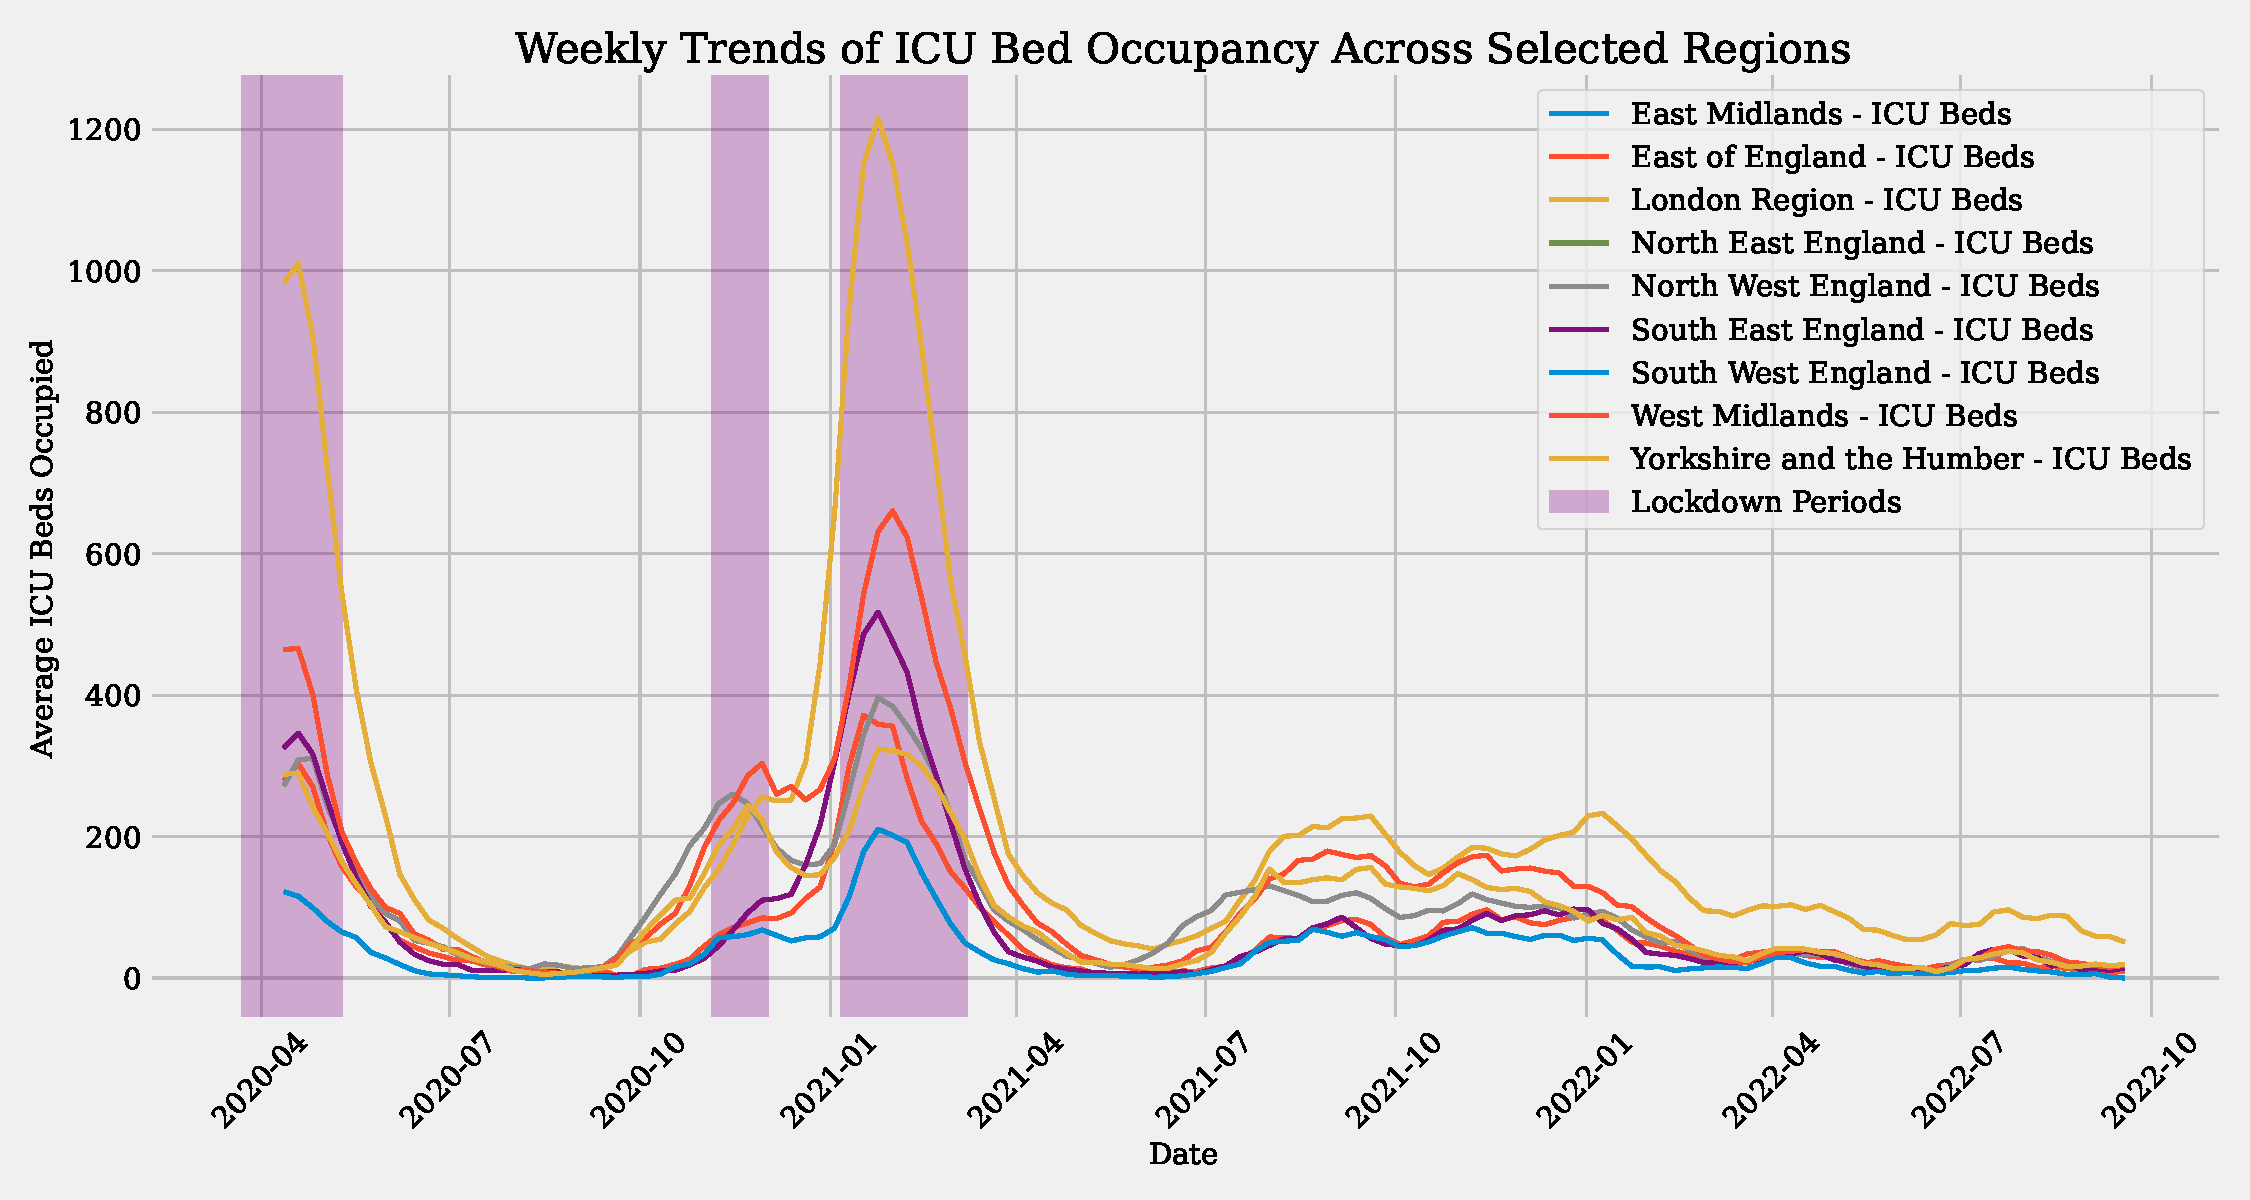
\includegraphics[width=0.8\textwidth]{"images/weekly_icu_beds_occupancy.pdf"}
    \caption{weekly ICU bed occupancy across NHS regions.}
    \label{fig:ICU_beds_occupancy}
\end{figure*}


\begin{figure*}[ht]
    \centering
    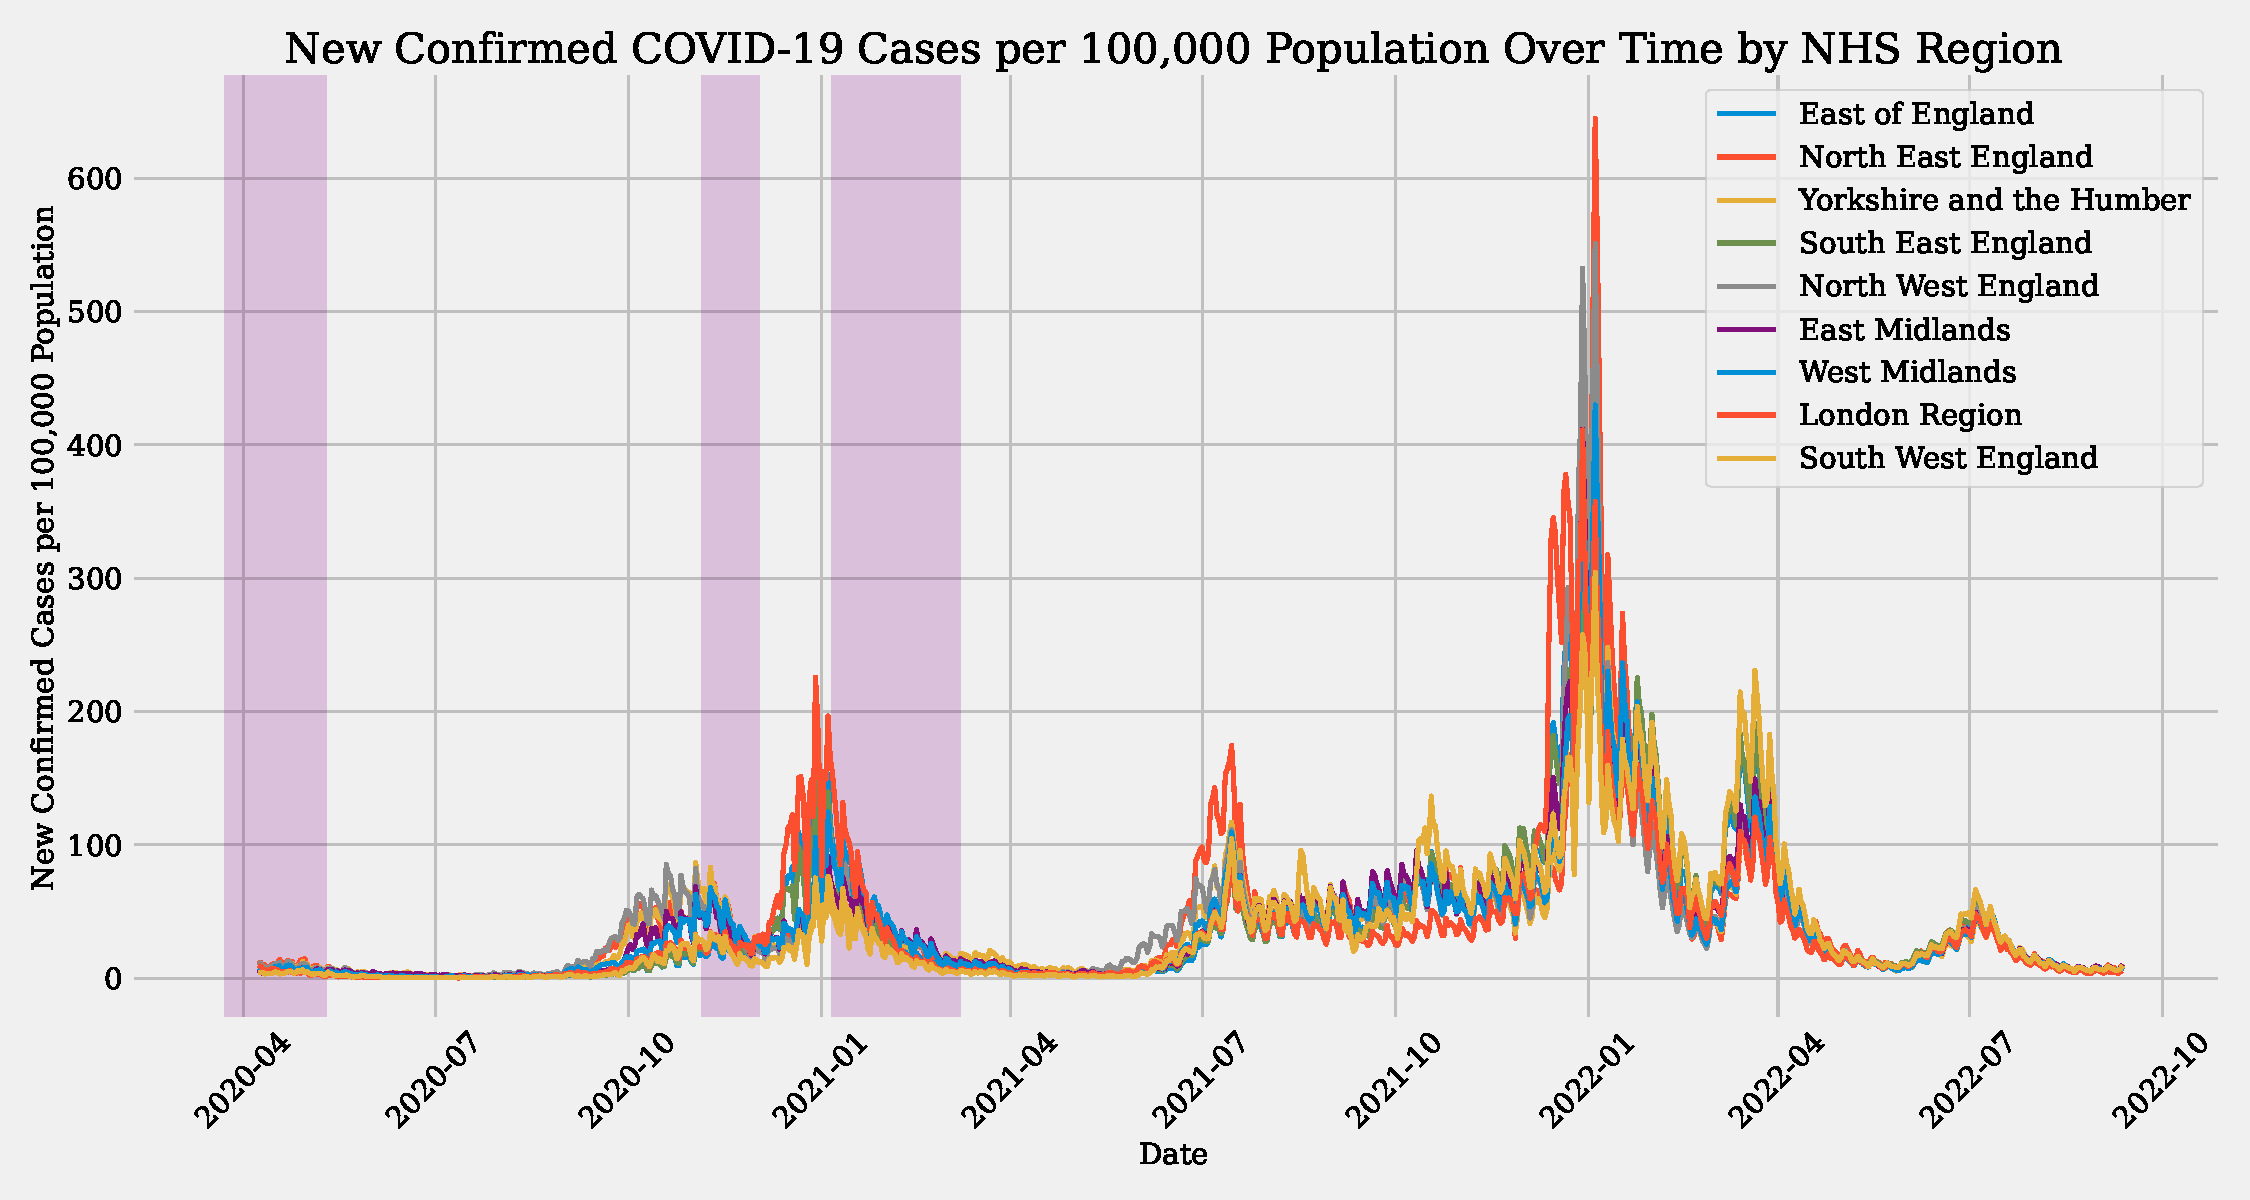
\includegraphics[width=0.8\textwidth]{"images/new_confirmed_per_100k.pdf"}
    \caption{new confirmed COVID-19 cases per 100k people overtime by NHS regions.}
    \label{fig:new_confirmed_per_100k}
\end{figure*}

\begin{figure*}[ht]
    \centering
    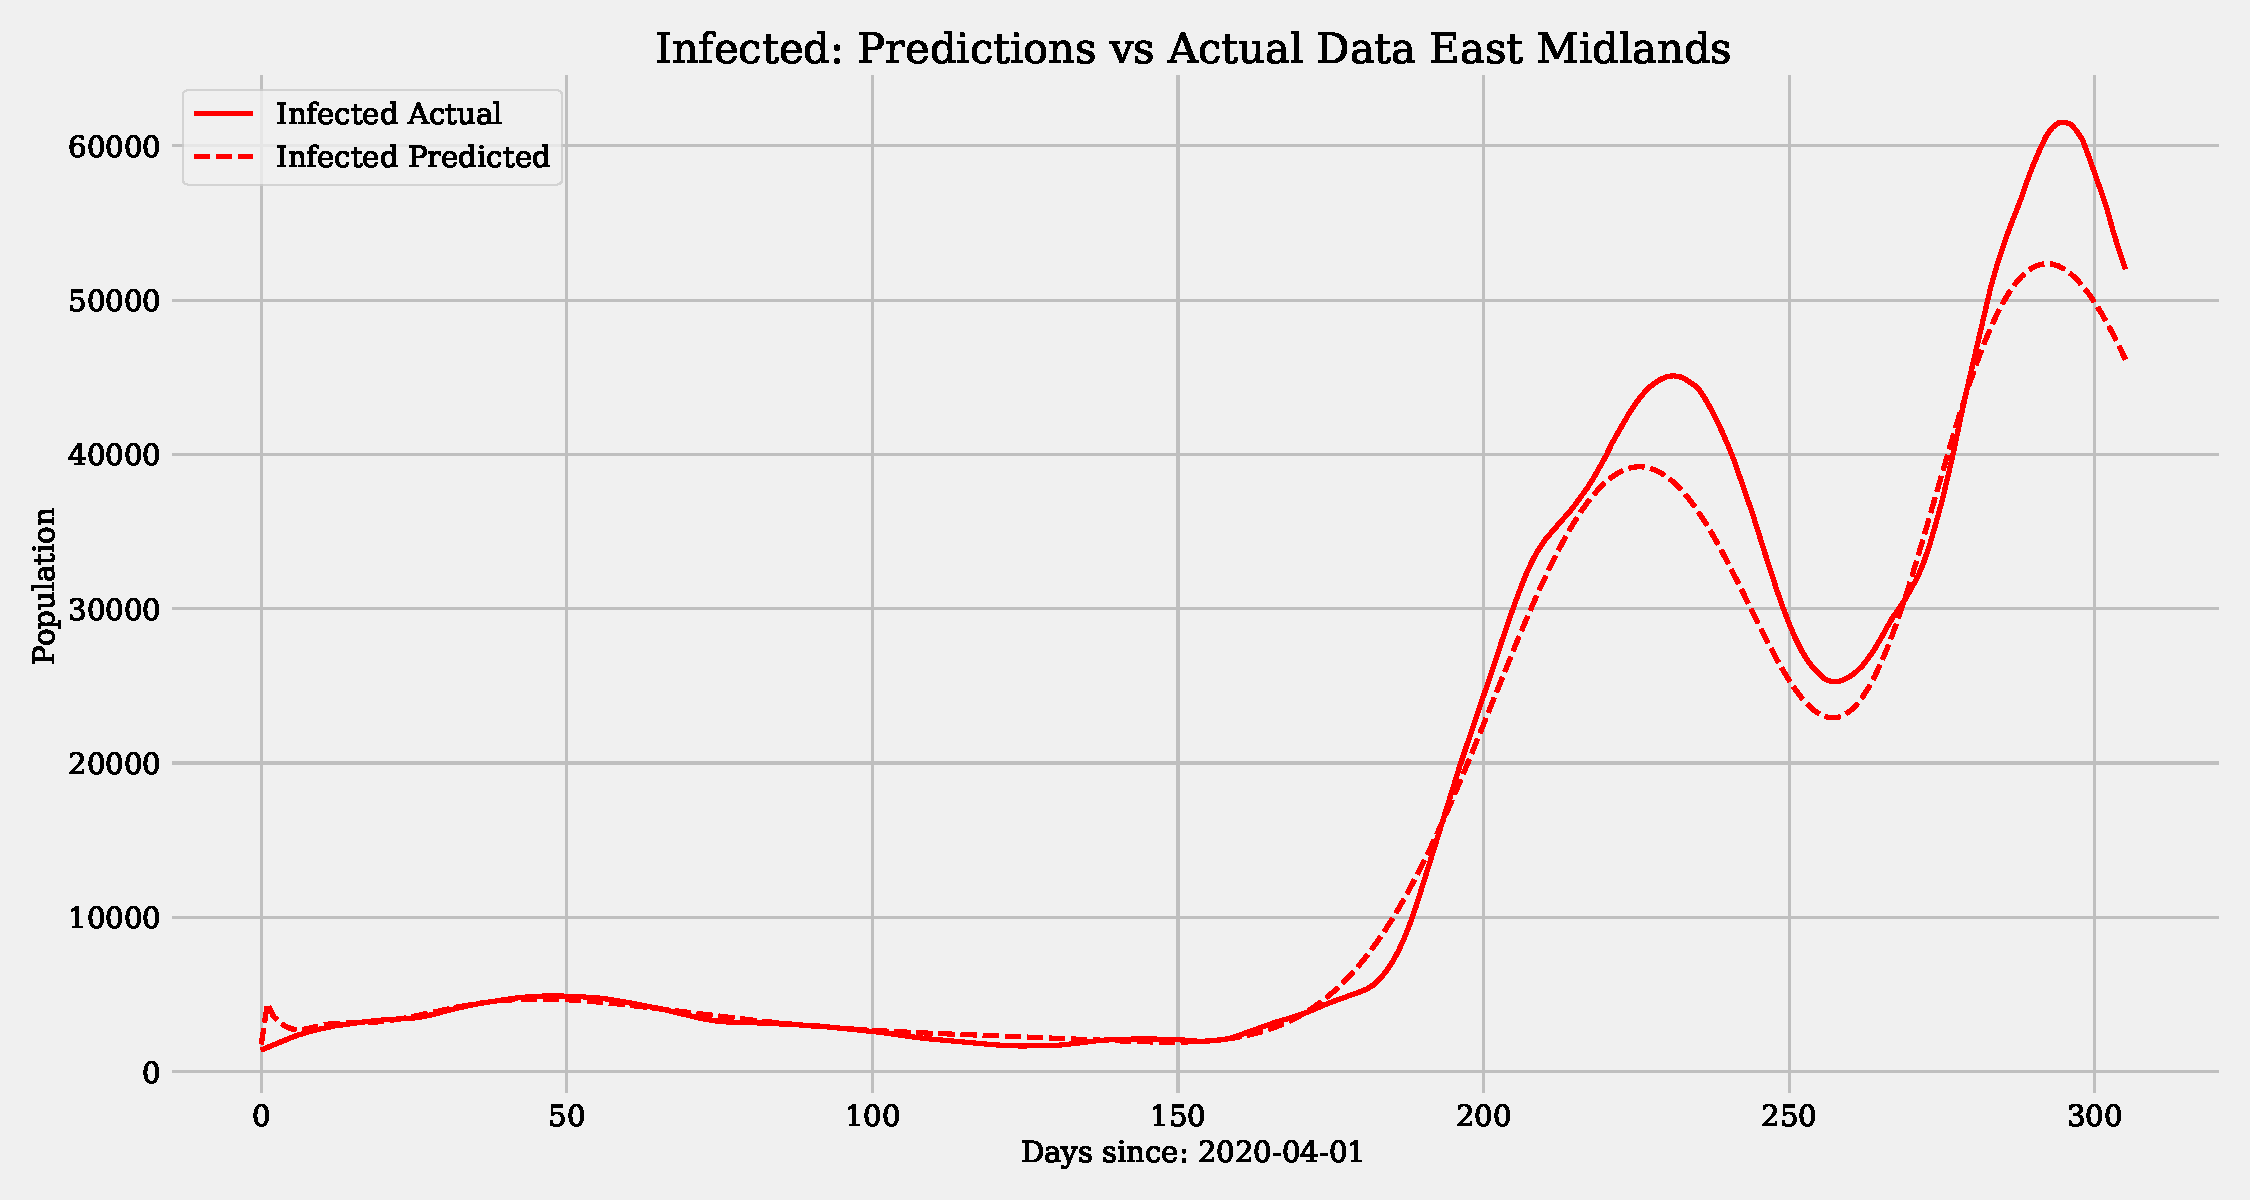
\includegraphics[width=0.8\textwidth]{images/pinn/I_predictions_East Midlands.pdf}
    \caption{Predicted number of infectious individuals in the East Midlands region.}
    \label{fig:I_predictions_East_Midlands}
\end{figure*}

\begin{figure*}[ht]
    \centering
    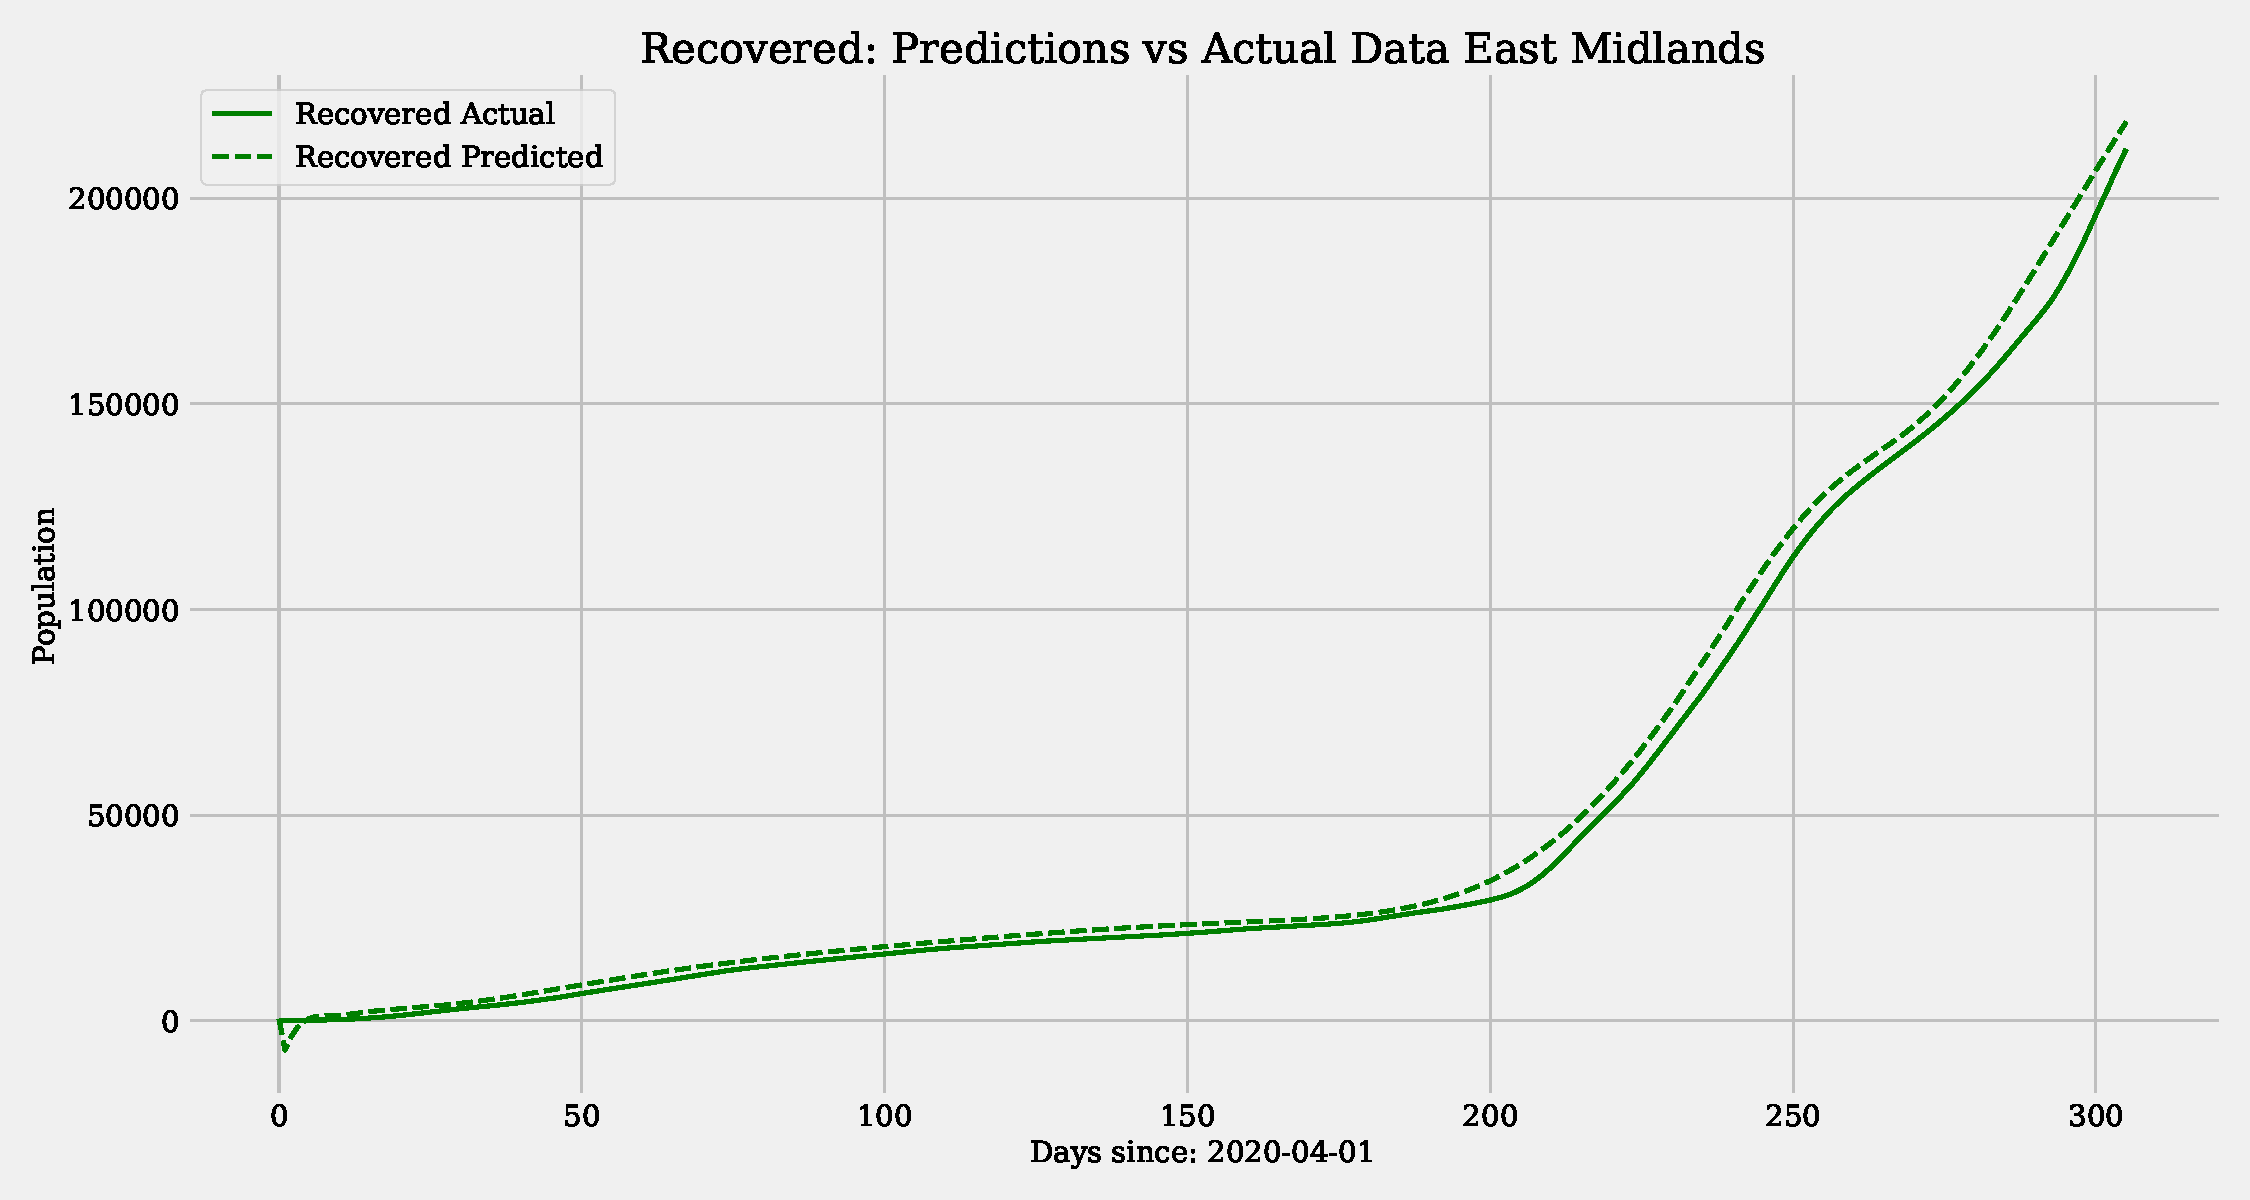
\includegraphics[width=0.8\textwidth]{images/pinn/R_predictions_East Midlands.pdf}
    \caption{Predicted number of recovered individuals in the East Midlands region.}
    \label{fig:R_predictions_East_Midlands}
\end{figure*}

\begin{figure*}[ht]
    \centering
    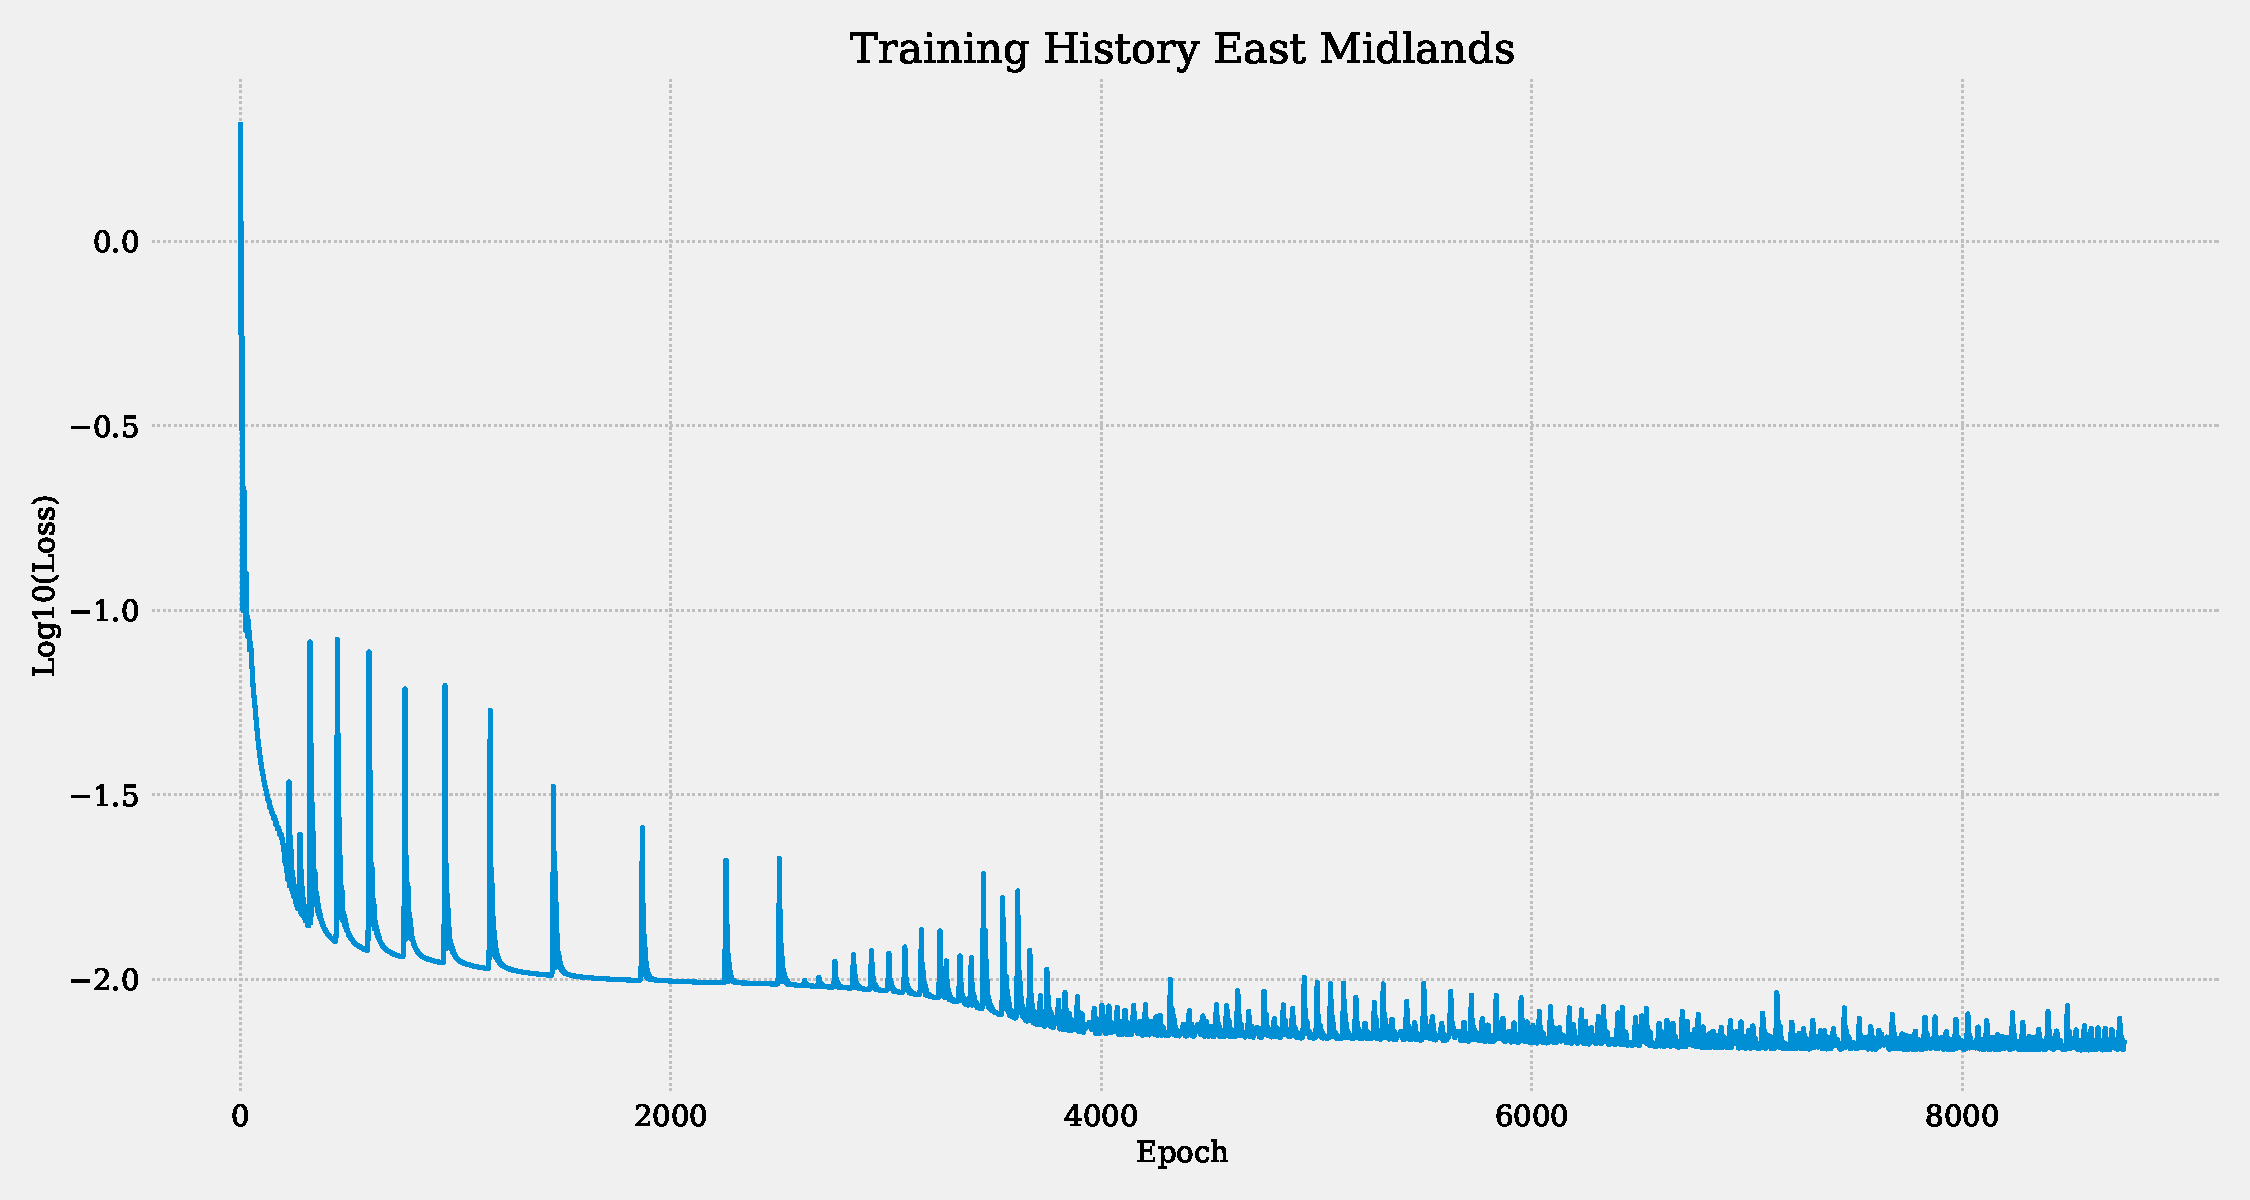
\includegraphics[width=0.8\textwidth]{images/pinn/Training_History_East Midlands.pdf}
    \caption{Training history of the PINN model for the East Midlands region.}
    \label{fig:Training_History_East_Midlands}
\end{figure*}

\begin{figure*}[ht]
    \centering
    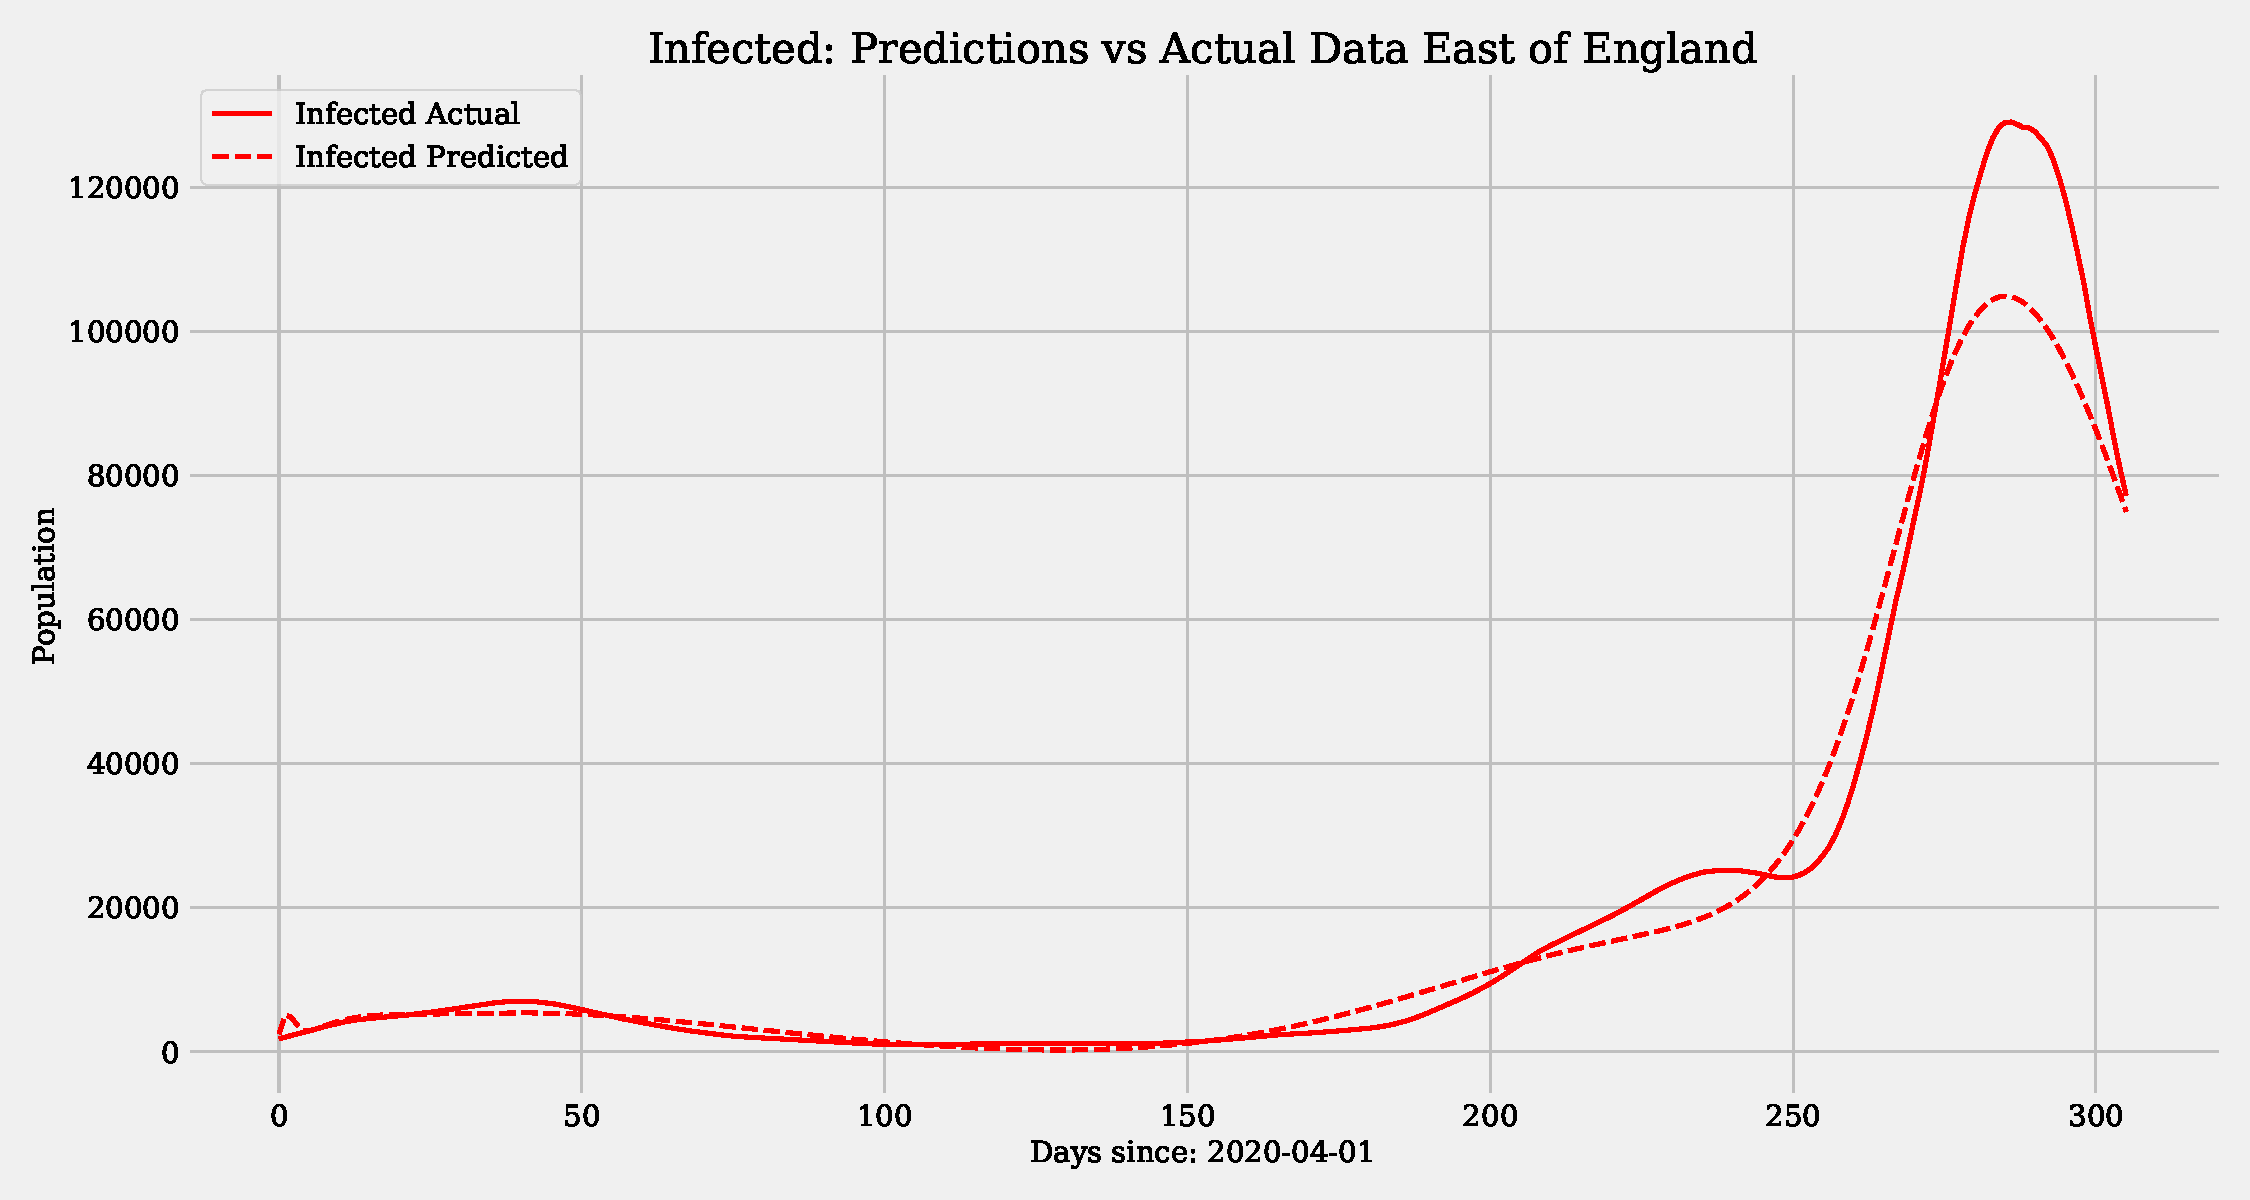
\includegraphics[width=0.8\textwidth]{images/pinn/I_predictions_East of England.pdf}
    \caption{Predicted number of infectious individuals in the East of England region.}
    \label{fig:I_predictions_East_of_England}
\end{figure*}

\begin{figure*}[ht]
    \centering
    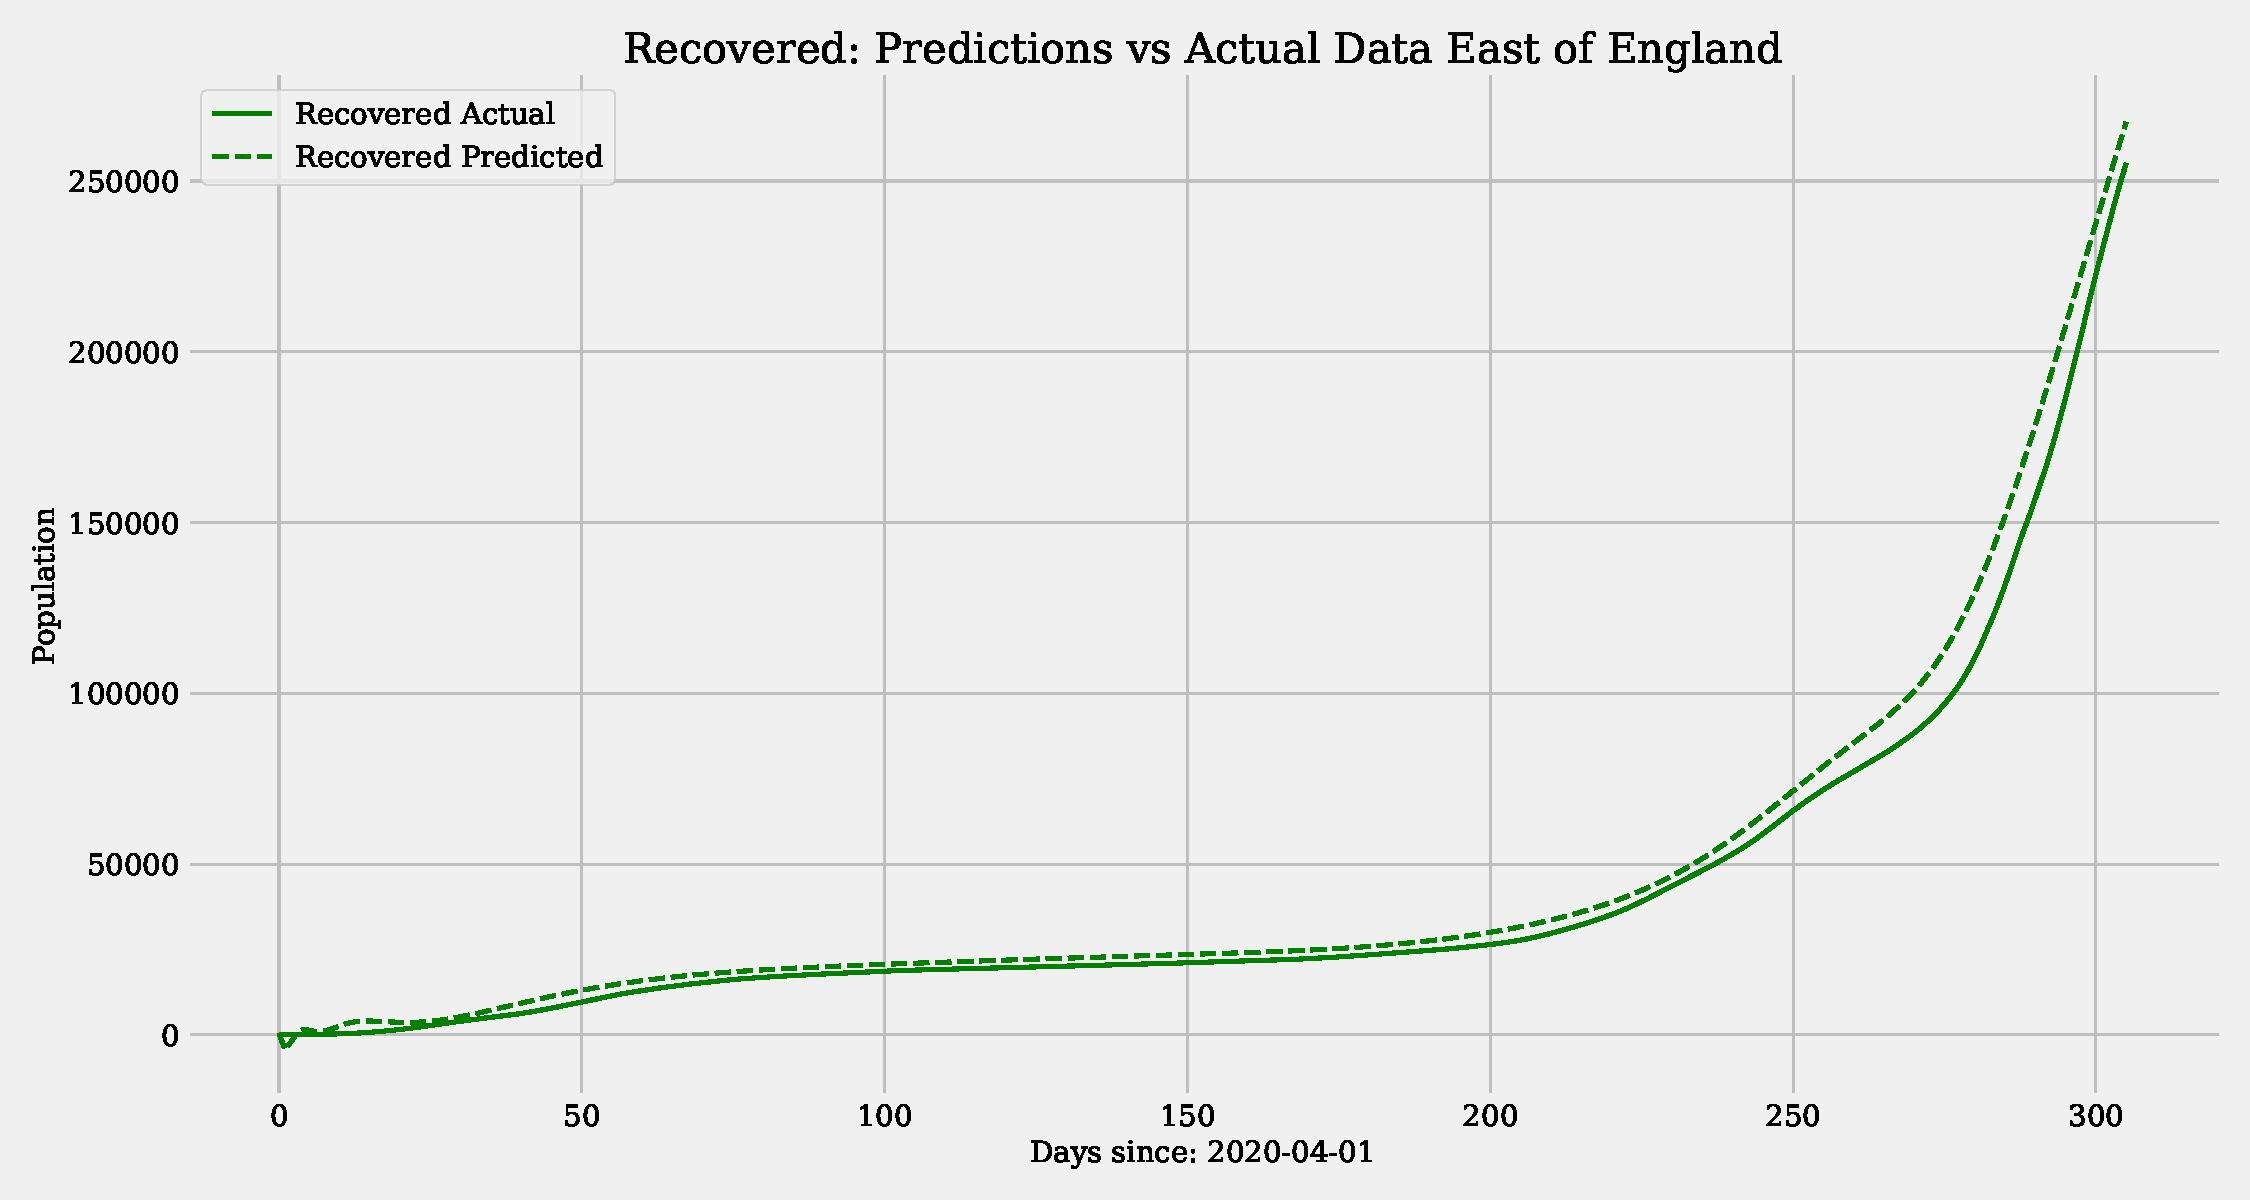
\includegraphics[width=0.8\textwidth]{images/pinn/R_predictions_East of England.pdf}
    \caption{Predicted number of recovered individuals in the East of England region.}
    \label{fig:R_predictions_East_of_England}
\end{figure*}

\begin{figure*}[ht]
    \centering
    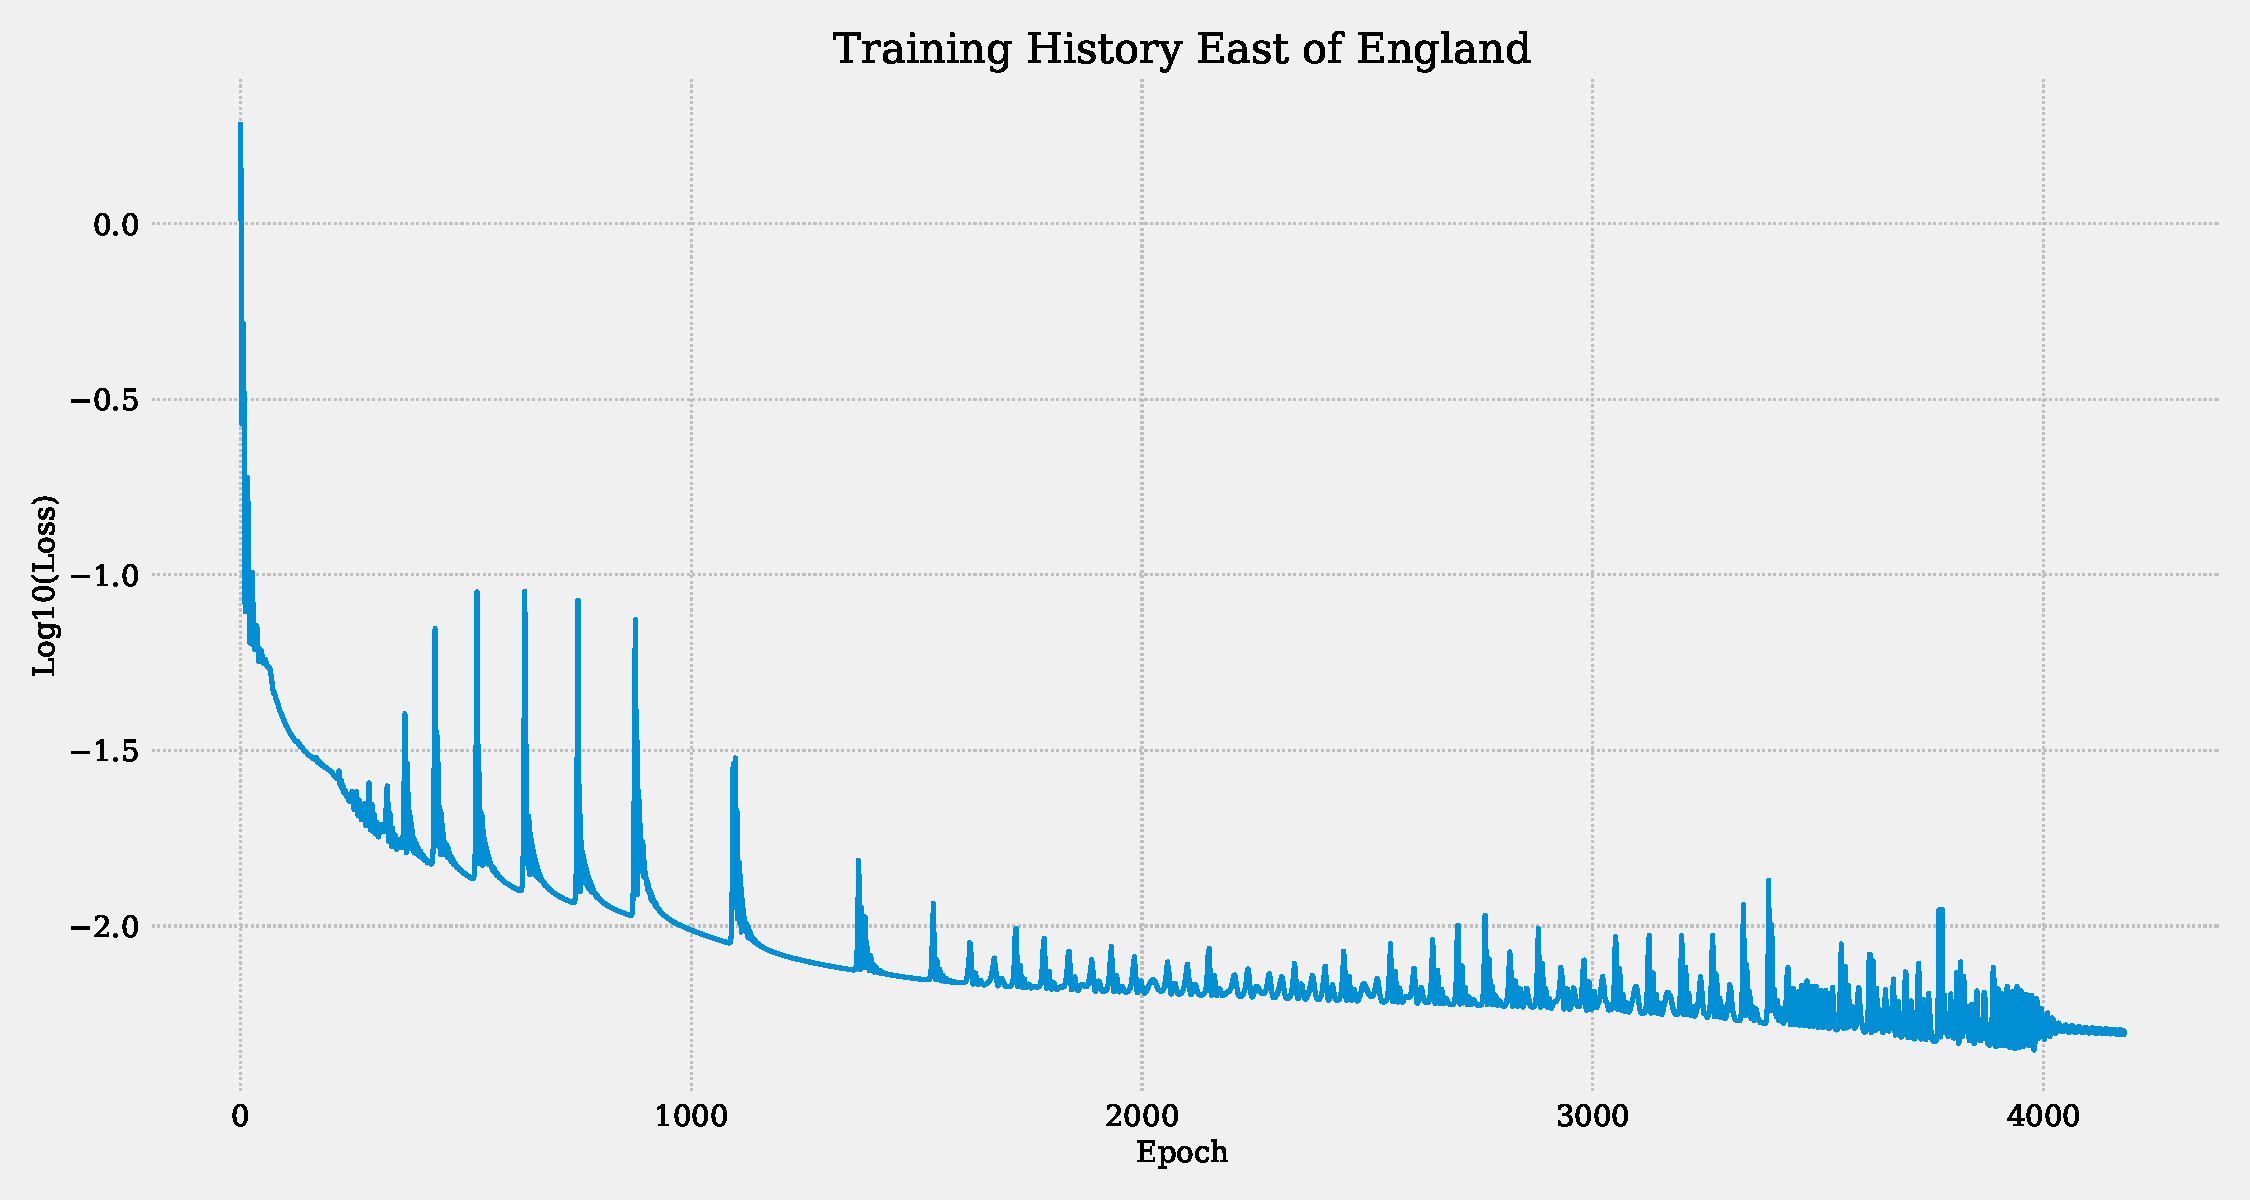
\includegraphics[width=0.8\textwidth]{images/pinn/Training_History_East of England.pdf}
    \caption{Training history of the PINN model for the East of England region.}
    \label{fig:Training_History_East_of_England}
\end{figure*}

\begin{figure*}[ht]
    \centering
    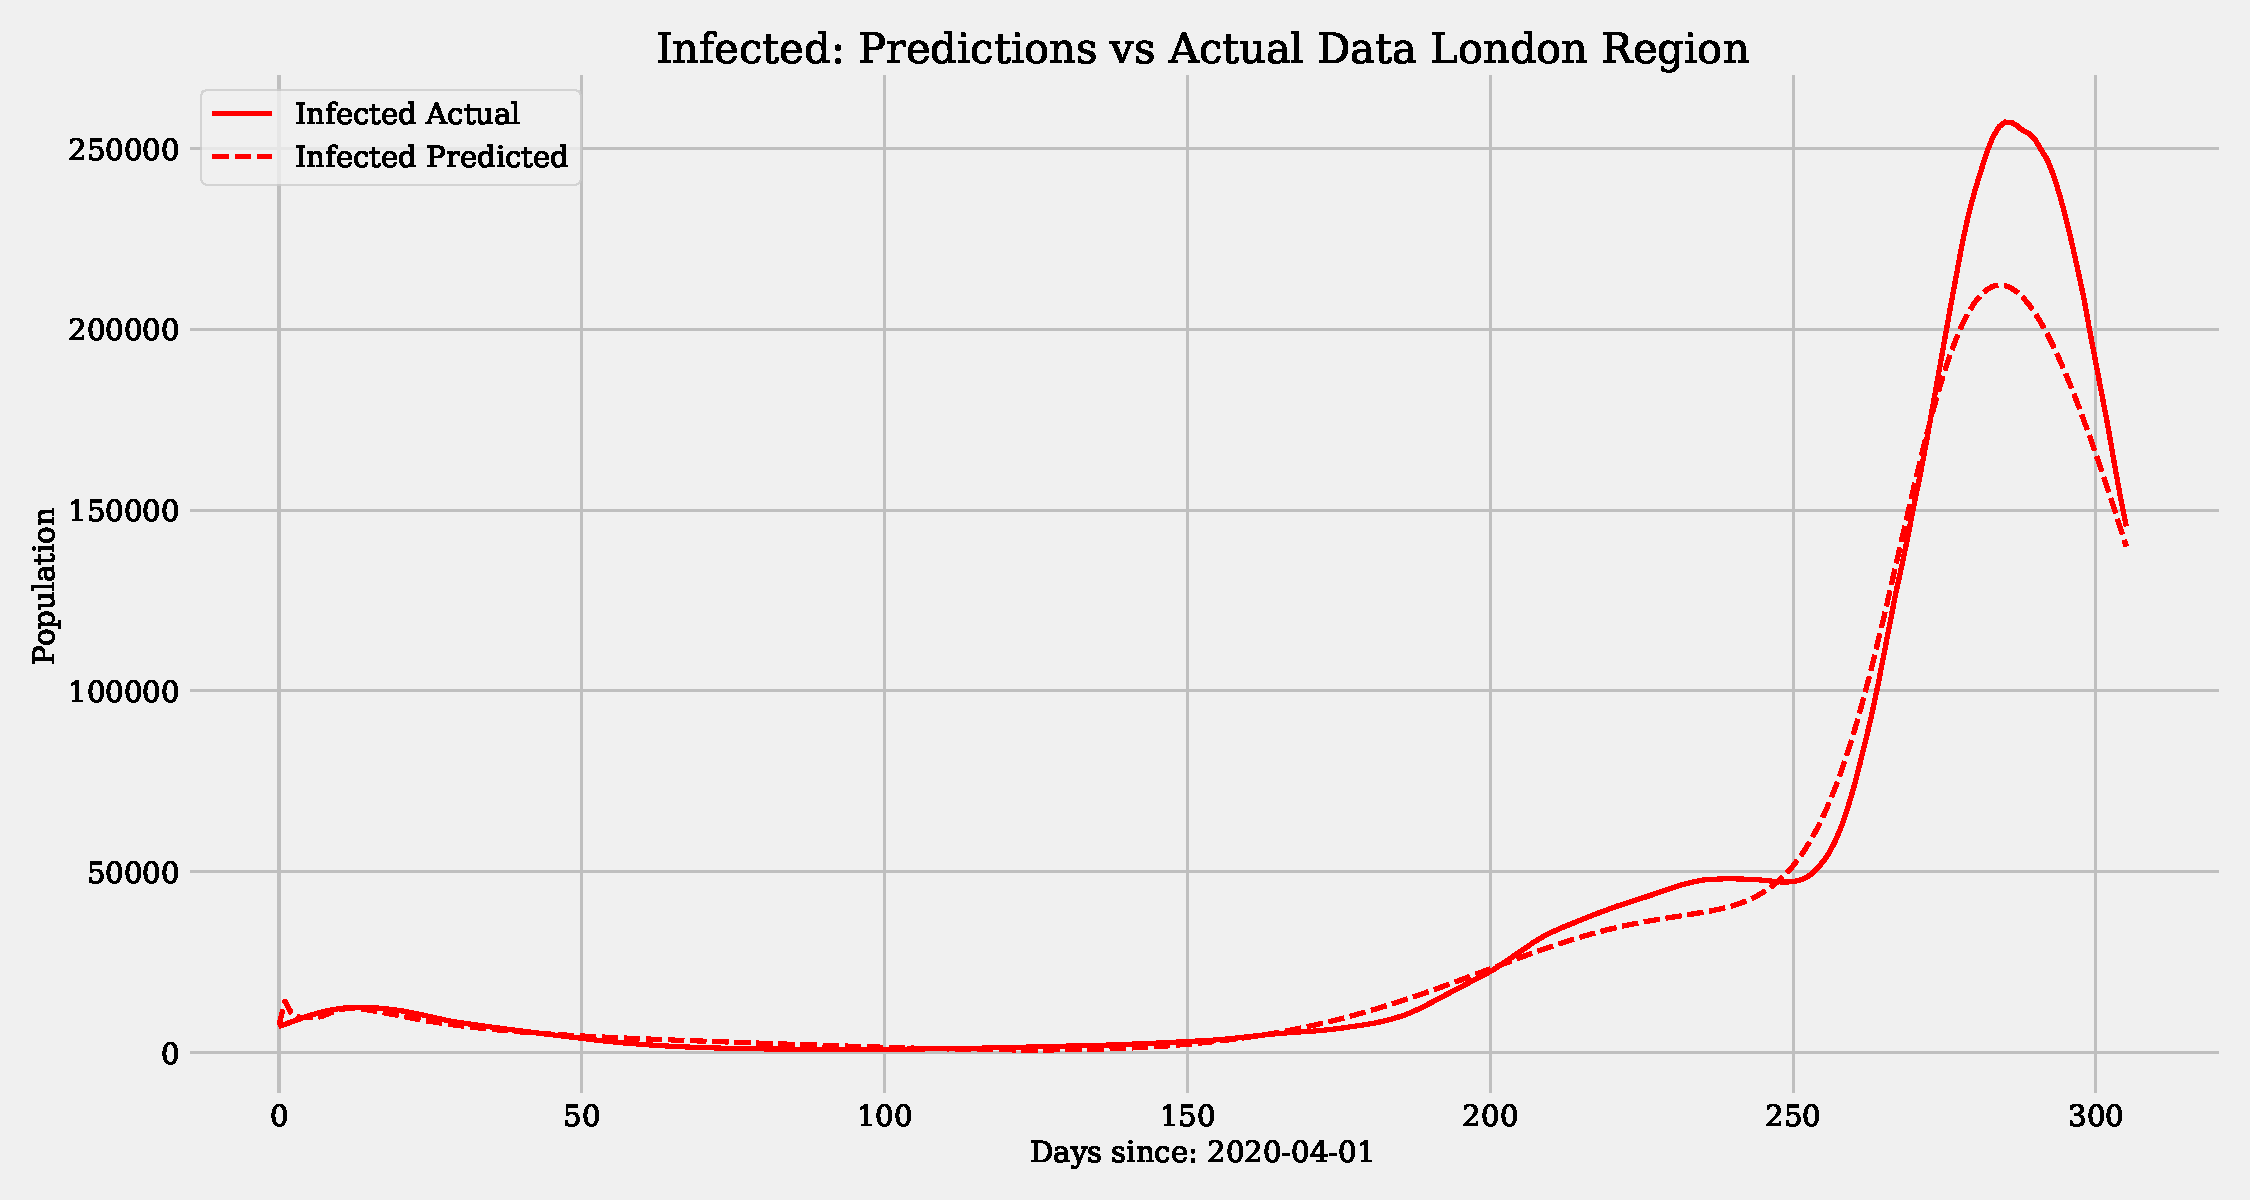
\includegraphics[width=0.8\textwidth]{images/pinn/I_predictions_London Region.pdf}
    \caption{Predicted number of infectious individuals in the London region.}
    \label{fig:I_predictions_London}
\end{figure*}

\begin{figure*}[ht]
    \centering
    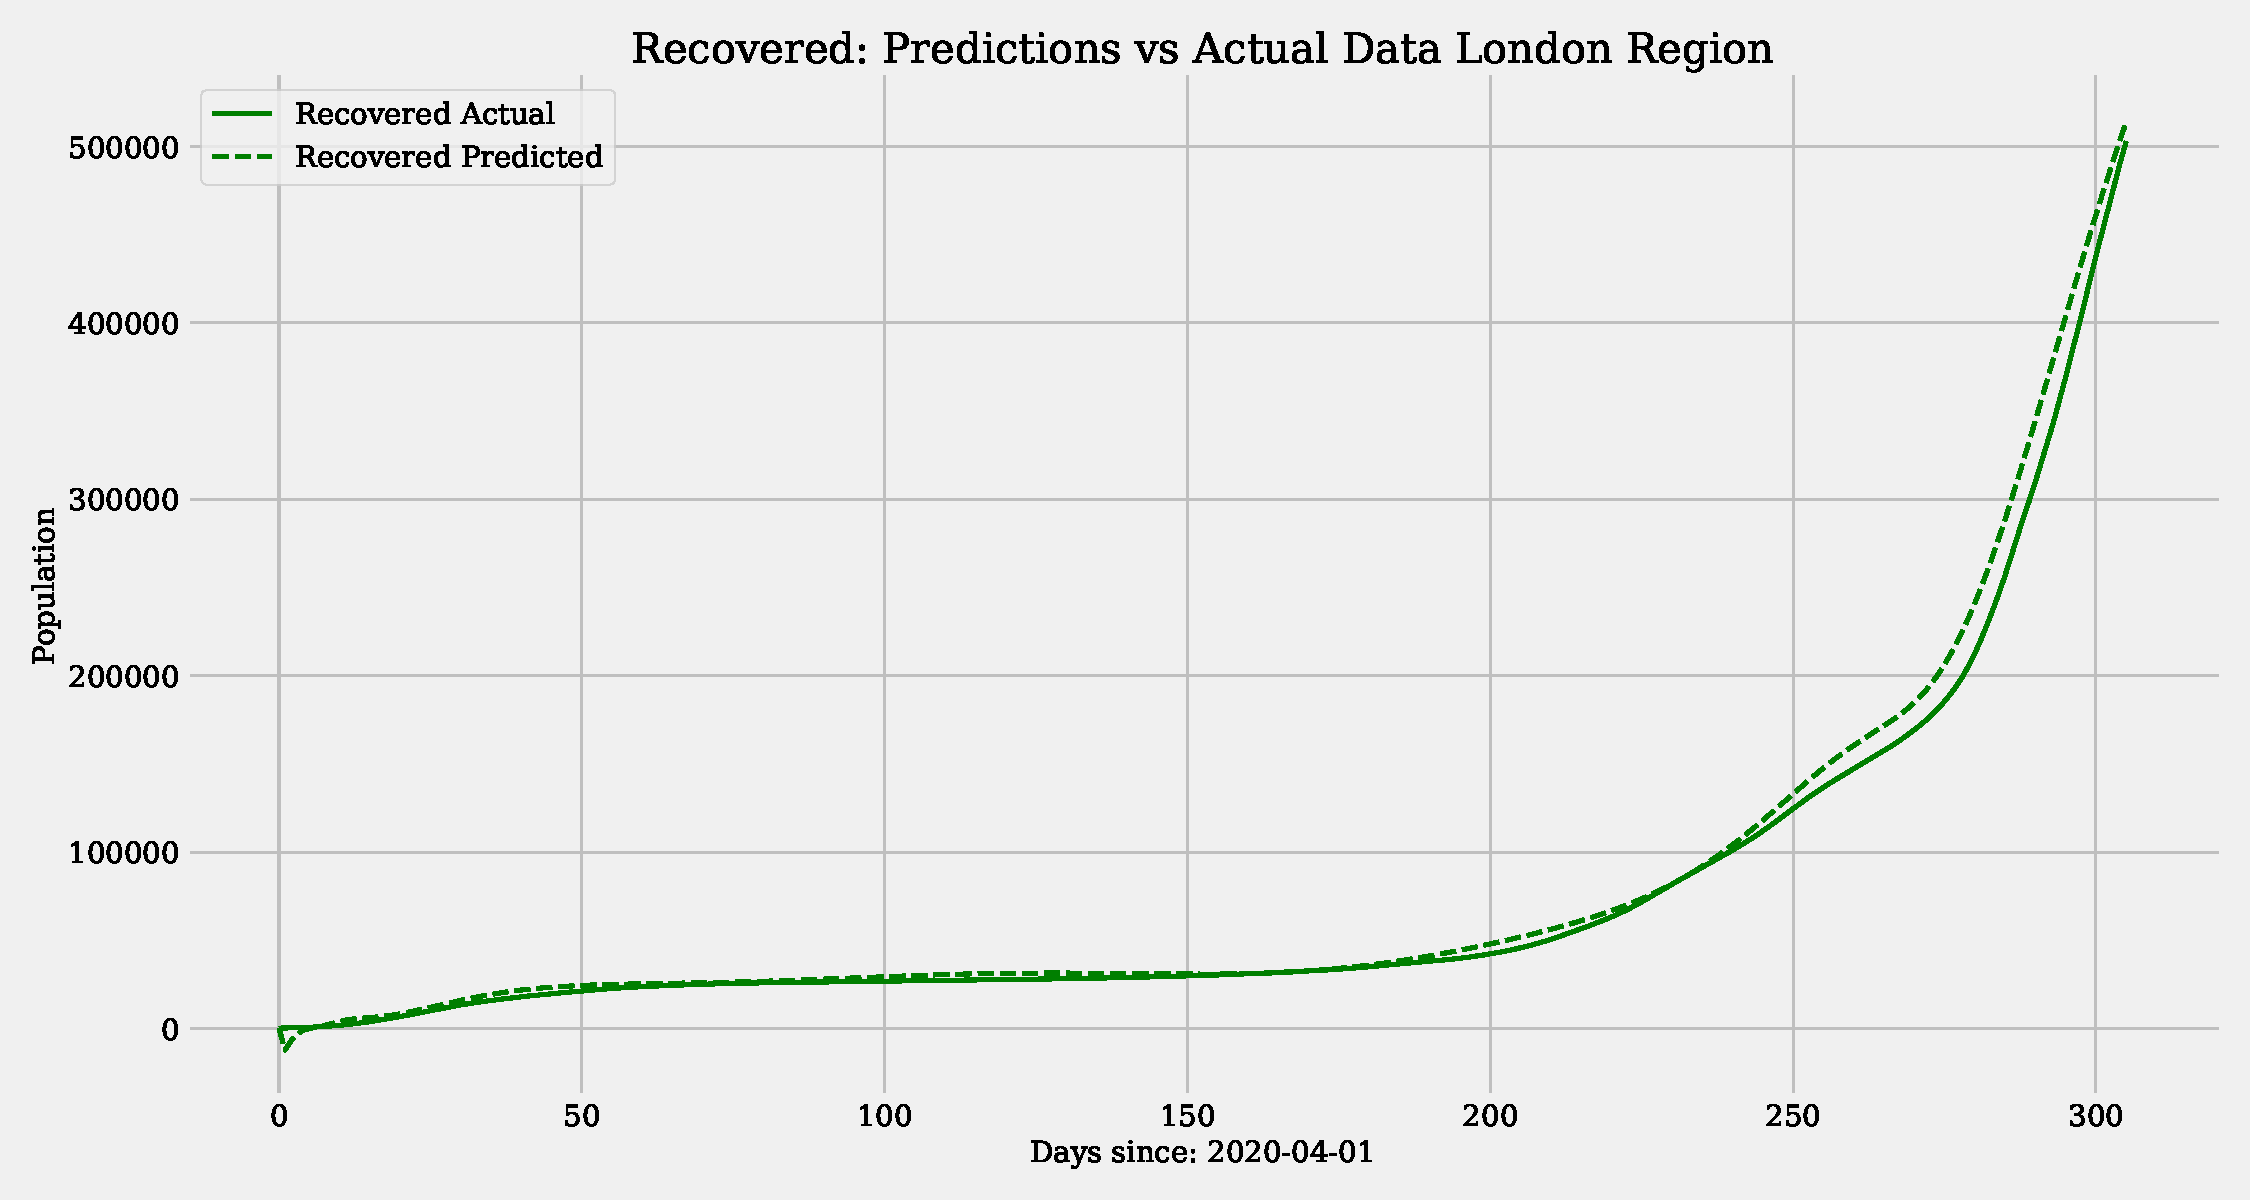
\includegraphics[width=0.8\textwidth]{images/pinn/R_predictions_London Region.pdf}
    \caption{Predicted number of recovered individuals in the London region.}
    \label{fig:R_predictions_London}
\end{figure*}

\begin{figure*}[ht]
    \centering
    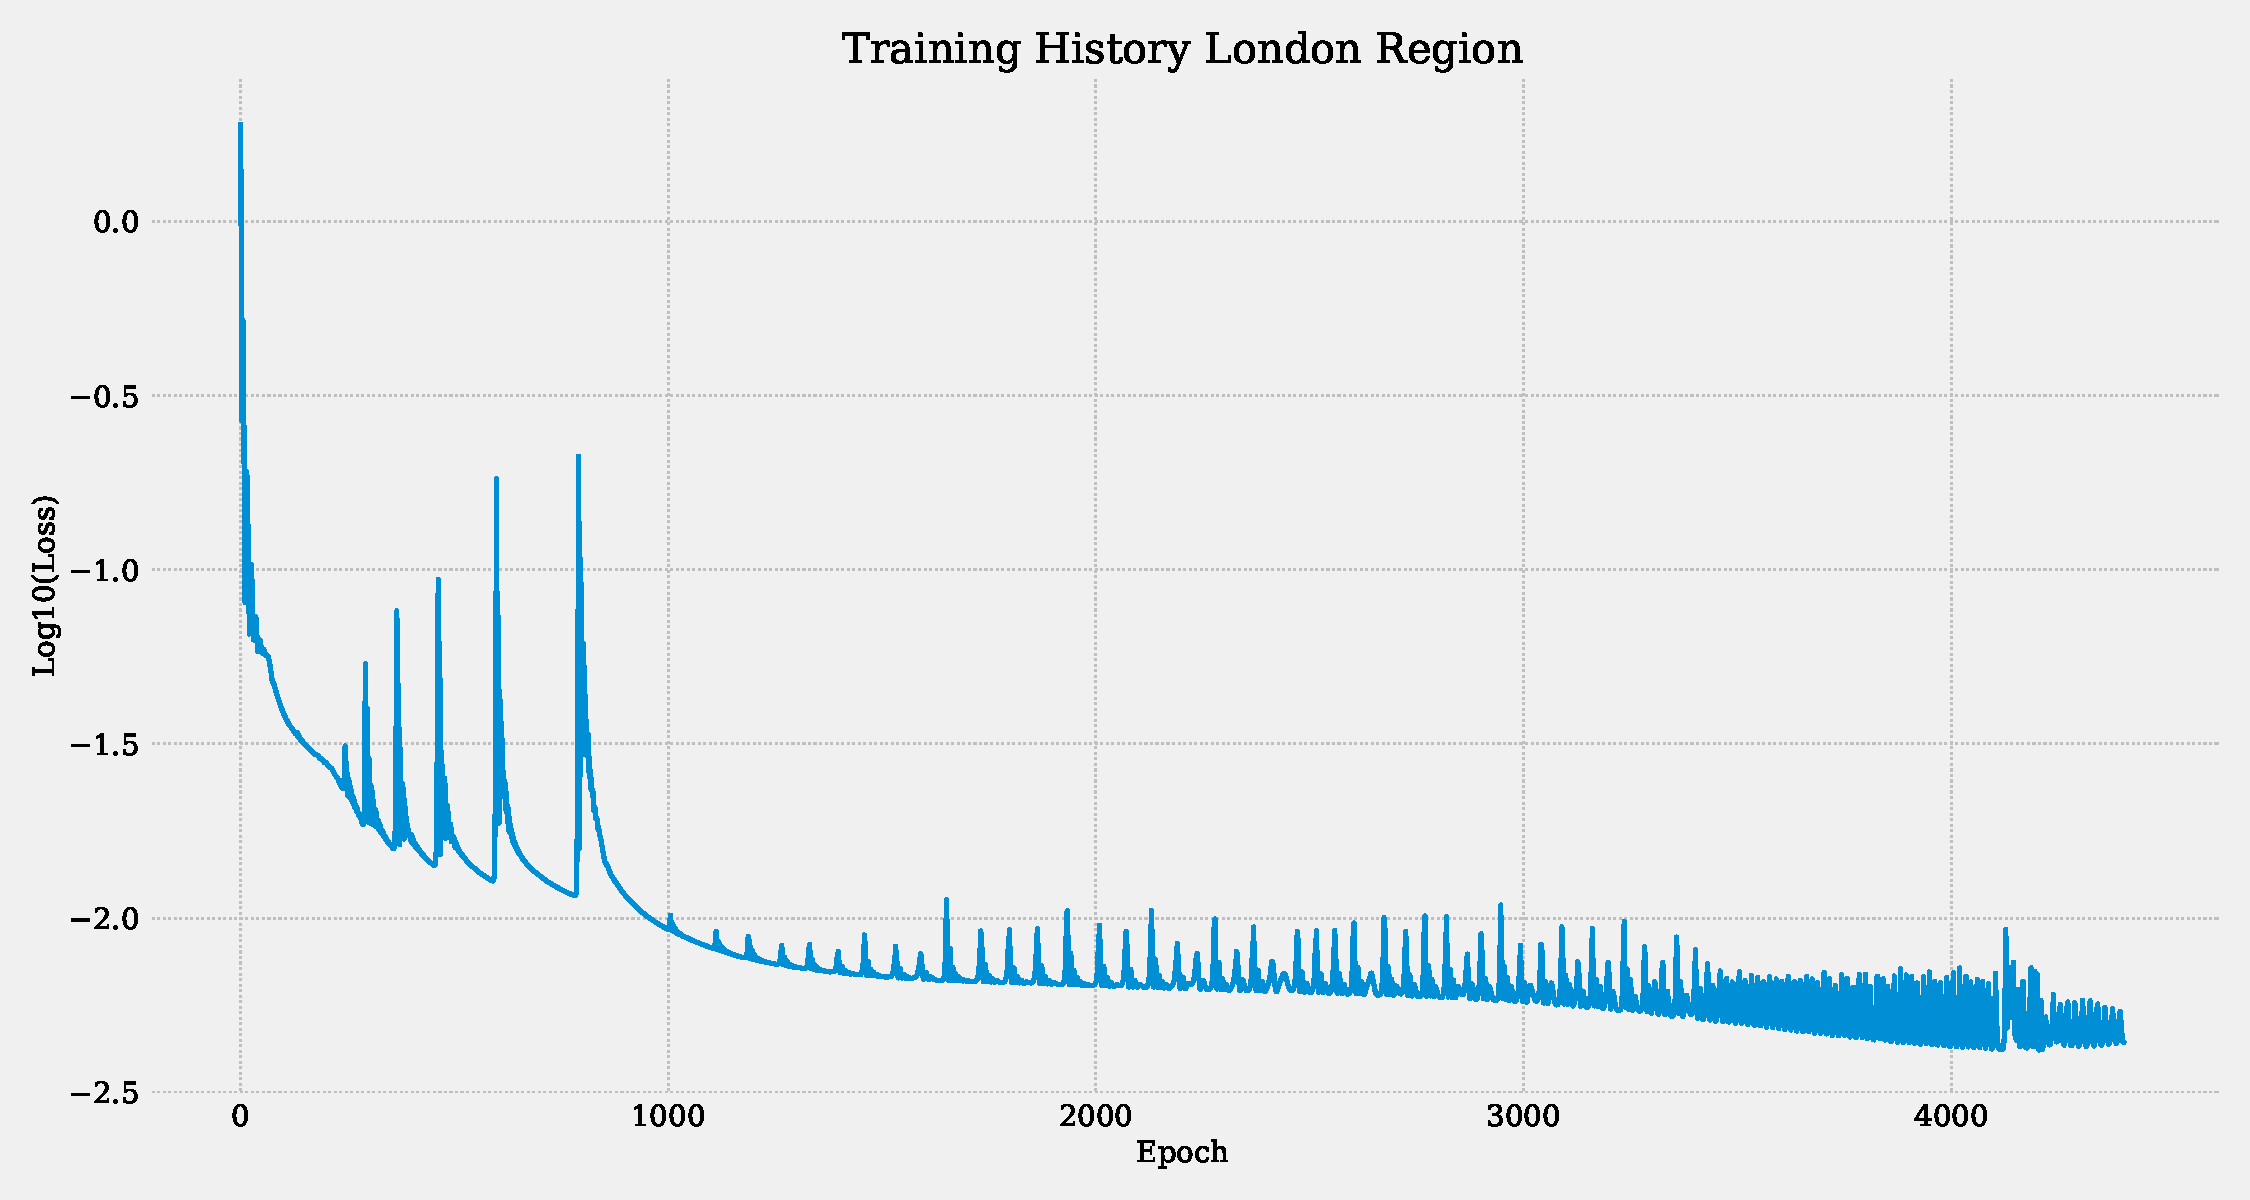
\includegraphics[width=0.8\textwidth]{images/pinn/Training_History_London Region.pdf}
    \caption{Training history of the PINN model for the London region.}
    \label{fig:Training_History_London}
\end{figure*}


\bibliographystyle{alphaurl}
\bibliography{refs}
\end{document}